\chapter{Generative invariants}
\label{chapter-gen}

So far in this thesis, we have presented \sls~as a framework for
presenting transition systems. This view focuses on synthetic
transitions as a way of relating pairs of process states, either with
one transition $(\Psi; \Delta) \leadsto (\Psi'; \Delta')$ or with a
series of transitions $(\Psi; \Delta) \leadsto^* (\Psi';
\Delta')$. This chapter will focus on another view of concurrent
\sls~specifications as {\it grammars} for describing well-formed
process states. This view was presented previously in the discussions
of adequacy in Section~\ref{sec:framework-reggenworld} and in
Section~\ref{sec:nat-ssos-adequacy}.

The grammar-like specifications that describe well-formed process
states are called {\it generative signatures}, and generative
signatures can be used to specify sets of process states, or {\it
  worlds}. By the analogy with grammars, we could also describe worlds
as {\it languages} of process states recognized by the grammar. In our
previous discussions of adequacy in
Section~\ref{sec:framework-reggenworld} and in
Section~\ref{sec:nat-ssos-adequacy}, the relevant world was a set of
process states that we could put in bijective correspondence with the
states of an abstract machine.

Our primary use of generative specifications in this thesis is showing
that, under some generative signature $\Sigma_{\it Gen}$ that defines
a world $\mathcal W$, whenever $(\Psi; \Delta) \in \mathcal W$ and
$(\Psi; \Delta) \leadsto_\Sigma (\Psi'; \Delta')$ it is always the
case that $(\Psi'; \Delta') \in \mathcal W$.  (The signature $\Sigma$
encodes the transition system we are studying.)  In such a case, the
world or language of well-formed process states is called a {\it
  generative invariant} of $\Sigma$.

\subsection*{Type preservation}

The purpose of this chapter is to demonstrate that generative
invariants are a solid methodology for describing invariants of
\sls~specifications, especially well-formedness and well-typedness
invariants of substructural operational semantics specifications like
the ones presented in Part II. As we have already
seen, well-formedness invariants are major part of adequacy
theorems. Well-typedness invariants are important because they allow us to
prove {\it language safety}, the property (discussed way back in the
introduction) that a language specification is completely free
from undefined behavior.

We don't generally expect all syntactically well-formed expressions
$\obj{e}$ to be free of undefined behavior. When we want to prove
language safety for a small-step SOS specification like $\obj{e
  \mapsto e'}$ from Section~\ref{sec:evaluationcontexts} and the
beginning of Chapter~\ref{chapter-absmachine}, we also define a
judgment $\obj{x_1{:}{\it tp_1},\ldots, x_n{:}{\it tp_n} \vdash e :
  {\it tp}}$.  This {\it typing judgment} expresses that $\obj{e}$ has
type $\obj{\it tp}$ if the expression variables $\obj{x_1, \ldots,
  x_n}$ are respectively assumed to have the types $\obj{\it tp_1,
  \ldots, tp_n}$. (Note that $\obj{\it tp}$ is an {\it object-level
  type} as described in Section~\ref{sec:gen-ordertp}, not an LF type
$\tau$ from Chapter~\ref{chapter-framework}.) Using the typing
judgment, we can prove the safety theorem -- all well-typed
expressions are free from undefined behavior -- by way of two
theorems. The first theorem is {\it preservation}: if $\obj{\cdot
  \vdash e : {\it tp}}$ and $\obj{e \mapsto e'}$ then $\obj{\cdot
  \vdash e' : {\it tp}}$. The second theorem is {\it progress}: if
$\obj{\cdot \vdash e : {\it tp}}$, then either there is some
$\obj{e'}$ such that $\obj{e \mapsto e'}$ or else $\obj{e}$ is already
a value.

Establishing a generative invariant for an SSOS language specification
is analogous to proving a preservation theorem in a small-step SOS
language specification. Progress and safety theorems for SSOS
specifications will be discussed in Chapter~\ref{chapter-safety}.
These two chapters establish the centerpiece of the third refinement
of our central thesis:

\smallskip
\begin{quote} 
  {\bf Thesis (Part III):} {\it The \sls~specification of the operational
    semantics of a programming language is a suitable basis for formal
    reasoning about properties of the specified language.}
\end{quote} 


\subsection*{Overview}

In Section~\ref{sec:gen-worlds} we review how generative signatures
define a world and show how the {\it regular worlds} that Sch\"urmann
implemented in Twelf \cite{schurmann00automating} fall out as a
special case of the worlds described by generative signatures.  We
will then discuss invariants of operationalized ordered abstract
machines, introduced in Section~\ref{sec:nat-ssos-adequacy}, more
generally (Section~\ref{sec:gen-order}). In
Section~\ref{sec:gen-ordertp} we will extend that discussion from
well-{\it formed} process states to well-{\it typed} process states.
This is not a large technical shift, but conceptually it is an
important step from thinking about adequacy properties to
thinking about preservation theorems. 
In Section~\ref{sec:gen-state}
we describe how generative invariants can be established for the sorts
of stateful signatures considered in
Section~\ref{sec:richer-ordered-abstract}. In
Section~\ref{sec:gen-destinations} we consider invariants for
specifications in the image of the destination-adding transformation
from Chapter~\ref{chapter-destinations}.  In
Section~\ref{sec:gen-letcc} we consider the peculiar case of
first-class continuations, which require us to use persistent
continuation frames as described in Section~\ref{sec:dest-continuations}. 
%Finally, in Section~\ref{sec:gen-count} we
%introduce a more complicated class of generative invariants that
%capture the numerical properties of specifications that appear in the
%\sls~encoding of voting and auction protocols.

All of these sections are essentially replaying the same
two-or-three-step proof with variations. The first step, which is not
always necessary, is reasoning about unique indices, a topic
introduced in Section~\ref{sec:uniqueness-genstate} and refined in
Section~\ref{sec:uniqueness-gendests}. The second step is to prove an
inversion lemma which allows us to gather knowledge about the last
steps of a generative trace based on our knowledge of the structure of
the generated process state. The third step is a preservation lemma
where we take in a generative trace, perform inversion upon it, and
then use the results of inversion to construct a new generative trace.

\section{Worlds}
\label{sec:gen-worlds}

{\it Worlds} are nothing more or less than sets of process states
$(\Psi; \Delta)$ -- in the discussion here, we will specifically
exclude process states $(\Psi; \Delta)_{\lf\sigma}$ with a non-empty
accompanying substitution $\lf\sigma$;\footnote{These accompanying
  substitutions were presented in
  Section~\ref{sec:sls-processstates}.} we don't need these
accompanying substitutions for any of the properties we want to
describe. 

In this chapter, we will specify worlds with the combination of two
artifacts: an initial process state and a generative signature.

\bigskip
\begin{definition}\label{def:gensig}
  A {\em generative signature} is a \sls~signature where the ordered,
  mobile, and persistent atomic propositions can be separated into two
  sets -- the {\em terminals} and the {\em nonterminals}. Synthetic
  transitions enabled by a generative signature only consume (or
  reference) nonterminals and LF terms, but their output variables can
  include LF variables, variables associated with terminals, and
  variables associated with nonterminals.
\end{definition}
\bigskip


\noindent
A generative signature, together with an initial
state $(\Psi_0; \Delta_0)$, describes a world with the help of the
restriction operator $\restrictsig{(\Psi; \Delta)}{\Sigma}$ introduced
in Section~\ref{sec:framework-restriction}. If $(\Psi; \Delta)$ is
well-defined under the generative signature $\Sigma_{\it Gen}$, and
$\Sigma$ is any signature that includes all of the generative
signature's terminals and all of its LF declarations but none of its
nonterminals, then $\restrictsig{(\Psi; \Delta)}{\Sigma}$ is only
defined when the only remaining nonterminals in $\Delta$ are
persistent and can therefore be filtered out of $\Delta$.  
%(As long as
%$\Sigma_{\it Gen}$ and $\Sigma$ have the same LF declarations, the LF
%context $\Psi$ won't have anything filtered out.) 
When the
classification of terminals and nonterminals is clear, we will leave
off the restricting signature and just write $\restrictsig{(\Psi;
  \Delta)}{}$. 

As a concrete example, let ${\sf nt/foo}$ be a persistent nonterminal,
let ${\sf nt/bar}$ be an ordered nonterminal, and let ${\sf t/baz}$ be
an ordered terminal. Then $\restrictsig{(x{:}\istrue{\susp{\sf
      nt/bar}}, y{:}\istrue{\susp{\sf t/baz}})}{}$ is undefined,
$\restrictsig{(y{:}\istrue{\susp{\sf t/baz}})}{} =
{(y{:}\istrue{\susp{\sf t/baz}})}$, and
$\restrictsig{(x{:}\ispers{\susp{\sf nt/foo}}, y{:}\istrue{\susp{\sf
      t/baz}})}{} = {(y{:}\istrue{\susp{\sf t/baz}})}$.  Recalling the
two-dimensional notation from Chapter~\ref{chapter-framework}, we can
re-present these three statements as follows:

\begin{center}
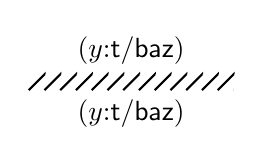
\begin{tikzpicture} 
\draw (.8,.5) node{$(y{:}\istrue{\susp{\sf t/baz}})$};
\draw [thick,dash pattern = on 2.82842842712mm off 2mm,decorate,decoration={saw,amplitude=2mm,segment length=2mm}] 
(-.5,0) -- (2.1,0); 
\draw (.8,-.3) node{$(y{:}\istrue{\susp{\sf t/baz}})$};
\end{tikzpicture} 
\quad
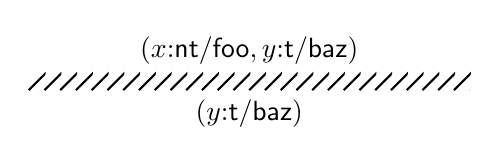
\begin{tikzpicture} 
\draw (.8,.5) node{$(x{:}\ispers{\susp{\sf nt/foo}},
  y{:}\istrue{\susp{\sf t/baz}})$};
\draw [thick,dash pattern = on 2.82842842712mm off 2mm,decorate,decoration={saw,amplitude=2mm,segment length=2mm}] 
(-2,0) -- (3.6,0); 
\draw (.8,-.3) node{$(y{:}\istrue{\susp{\sf t/baz}})$};
\end{tikzpicture}
\quad
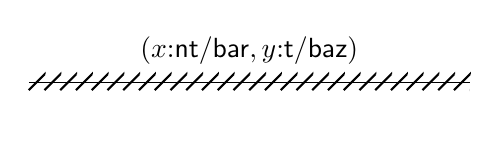
\begin{tikzpicture} 
\draw (.8,.5) node{$(x{:}\istrue{\susp{\sf nt/bar}},
  y{:}\istrue{\susp{\sf t/baz}})$};
\draw [thick,dash pattern = on 2.82842842712mm off 2mm,decorate,decoration={saw,amplitude=2mm,segment length=2mm}] 
(-2,0) -- (3.6,0); 
\draw (-2,.1) -- (3.6,.1); 
\draw (.8,-.3) node{\color{white} $(y{:}\istrue{\susp{\sf t/baz}})$};
\end{tikzpicture} 
\end{center}


Definition~\ref{def:gensig} is intentionally quite broad -- it need
not even be decidable whether a process state belongs to a particular
world.\footnote{Proof: consider the initial state
  $(x{:}\istrue{\susp{\sf gen}})$ and the rule $\forall
  \lf{e}.\,\forall\lf{v}.\,{\sf gen} \fuse {!}({\sf
    ev}\,\lf{e}\,\lf{v}) \lefti \{ {\sf terminating}\,\lf{e} \}$. The
  predicate ${\sf gen}$ is a nonterminal, the predicate ${\sf
    terminating}$ is a terminal, and ${\sf ev}$ is the encoding of
  big-step evaluation $\obj{e \Downarrow v}$ from
  Figure~\ref{fig:example-transform-cbv}.  The language described is
  isomorphic to the set of $\lambda$-calculus expressions that terminate
  under a call-by-value strategy,
  and membership in that set is undecidable.} Future tractable
analyses will therefore presumably be based upon further restrictions
of the very general Definition~\ref{def:gensig}.  Context-free
grammars are one obvious specialization of generative signatures; we
used this correspondence as an intuitive guide in
Section~\ref{sec:framework-reggenworld}.  Perhaps less obviously,
the regular worlds of Twelf \cite{schurmann00automating} are another
specialization of generative signatures.


\subsection{Regular worlds}
\label{sec:gen-regularworlds}

The
regular world specifications used in Twelf
\cite{schurmann00automating} are made up of {\it blocks}. A block
describes a little piece of an LF context, and is declared in the LF
signature as follows:
\[
 {\sf blockname} :
 {\sf some}~\{\lf{a_1}{:}\tau_1\}\ldots\{\lf{a_n}{:}\tau_n\}
~{\sf block}~\{\lf{b_1}{:}\tau'_1\}\ldots\{\lf{b_m}{:}\tau'_m\}
\]
A block declaration is well formed in the signature $\Sigma$ if, 
by the definition of well-formed signatures from Figure~\ref{fig:lf-form}, 
$\cdot \vdash_\Sigma \lf{a_1}{:}\tau_1,\ldots,\lf{a_{n}}{:} \tau_{n}\,{\sf ctx}$
and 
$\lf{a_1}{:}\tau_1,\ldots,\lf{a_{i-1}}{:} \tau_{n}
  \vdash_\Sigma \lf{b_1}{:}\tau'_1,\ldots,\lf{b_{m}}{:}\tau'_{m} \,{\sf ctx}$.

The first list of LF variable bindings
$\{\lf{a_1}{:}\tau_1\}\ldots\{\lf{a_n}{:}\tau_n\}$ that 
come after the ${\sf some}$ keyword describe the types
of concrete LF terms that must exist for the block to be well formed.
The second list of LF variable bindings represents the bindings that
the block actually adds to the LF context. The regular worlds of 
Twelf are defined as sets of block identifiers 
$({\sf block1} \mid \ldots \mid {\sf blockn})$. A set of block identifiers
and a Twelf signature $\Sigma$ inductively define a world as follows: if
\smallskip
\begin{itemize}
\item $\Psi$ is a well-formed
LF context in the current world, 
\item ${\sf blockname} :
 {\sf some}~\{\lf{a_1}{:}\tau_1\}\ldots\{\lf{a_n}{:}\tau_n\}
~{\sf block}~\{\lf{b_1}{:}\tau'_1\}\ldots\{\lf{b_m}{:}\tau'_m\} \in \Sigma$
 is one of the blocks in the current world, and
\item there is a $\lf{\sigma}$ such that
$\Psi \vdash_\Sigma \lf{\sigma} :
\lf{a_1}{:}\tau_1,\ldots,\lf{a_n}{:}\tau_n$, 
\end{itemize}
\smallskip then $\Psi, \lf{b_1}{:}\lf\sigma\tau'_1,\ldots,
\lf{b_m}{:}\lf\sigma\tau'_m$ is also a well-formed LF context in the
current world. The {\it closed world}, containing no variables at all,
 is a subset of every regular world, so this definition
gives us the rules for generating a world -- a set of contexts -- from
a series of block declarations.

One simple example of a regular world (previously discussed in
Section~\ref{sec:framework-reggenworld}) is the world that just
contains arbitrary expression variables with LF type ${\sf exp}$. This
world can be described with the block ${\sf blockexp}$:
\[
 {\sf blockexp} : 
 {\sf some}
~{\sf block}~\{{\lf x}{:}{\sf exp}\}
\]
If we had a judgment ${\sf natvar}\,\lf{x}\,\lf{n}$ that associated
every LF variable $\lf{x}{:}{\sf exp}$ with some natural number
$\lf{n}{:}{\sf nat}$, then in order to make sure that every expression
variable was associated with some natural number we would use the world
described by this block:
\[
 {\sf blocknatvar} : 
 {\sf some}~\{{\lf n}{:}{\sf nat}\}
~{\sf block}~\{{\lf x}{:}{\sf exp}\}~
               \{\lf{\it nv}{:}{\sf natvar}\,\lf{x}\,\lf{n}\}
\]
The world described by the combination of ${\sf blockexp}$ and ${\sf
  blocknatvar}$ is one where every LF variable $\lf{x}{:}{\sf exp}$ is
associated with at most one LF variable of type ${\sf
  natvar}\,\lf{x}\,\lf{n}$. Assuming that there are no constants of
type ${\sf natvar}$,\footnote{This is a property we can easily enforce
  with subordination, which was introduced in
  Section~\ref{sec:framework-lf-judgments}.} this gives us a
uniqueness property: if ${\sf natvar}\,\lf{x}\,\lf{n}$ and ${\sf
  natvar}\,\lf{x}\,\lf{m}$, then $\lf{m} = \lf{n}$.

\subsection{Regular worlds from generative signatures}

A block declaration ${\sf blockname} :
 {\sf some}~\{\lf{a_1}{:}\tau_1\}\ldots\{\lf{a_n}{:}\tau_n\}
~{\sf block}~\{\lf{b_1}{:}\tau'_1\}\ldots\{\lf{b_m}{:}\tau'_m\}$ can
be described by one rule in a generative signature:
\begin{align*}
&{\sf blockname} : 
  \forall \lf{a_1}{:}\tau_1\ldots \forall\lf{a_n}{:}\tau_n.\,
  \{ \exists \lf{b_1}{:}\tau'_1 \ldots \lf{b_m}{:}\tau'_m.\,
     \one
  \}
\intertext{Because a regular world is just a set of blocks, 
the generative signature corresponding
to a regular world contains one rule for each block in the regular
worlds description.
The world $({\sf blockexp} \mid {\sf blockvar})$ corresponds
to the following generative signature:}
&{\sf nat} : {\sf type}, 
\\
&\mbox{\it \ldots declare constants of type ${\sf nat}$ \ldots }
\\
&{\sf exp} : {\sf type}, 
\\
&\mbox{\it \ldots declare constants of type ${\sf exp}$ \ldots }
\\
&{\sf blockexp} : 
  \{ \exists \lf{x}{:}{\sf exp}.\,\one\},
\\
&{\sf blocknatvar} : \forall \lf{n}{:}{\sf nat}.\,
  \{ \exists \lf{x}{:}{\sf exp}.\,
     \exists \lf{\it nv}{:}{\sf natvar}\,\lf{x}\,\lf{n}.\, \one \}
\end{align*}
Call this regular world signature $\Sigma_{\it RW}$. It is an extremely
simple example of a generative signature -- there are no
terminals and no nonterminals -- so the restriction operator has
no effect. The world described by $({\sf blockexp} \mid {\sf blocknatvar})$
is identical to the set of LF contexts $\Psi$ such that
$(\cdot; \cdot) \leadsto_{\Sigma_{RW}} (\Psi; \cdot)$.

\subsection{Regular worlds in substructural specifications}

From the structure of translated LF regular worlds, it is hopefully
apparent that by replacing the proposition $\one$ in the heads of the
generative ${\sf block*}$ rules with less trivial positive 
\sls~propositions. In this way, we can extend the language of regular
worlds to allow the introduction of ordered, mobile, and persistent
\sls~propositions as well. For instance, the rule
${\sf blockitem} : 
\forall \lf{n}. \, \{ {\sf item}\,\lf{n} \}$,
where ${\sf item}$ is a mobile predicate,
describes the world of contexts that take the form
$\left(\cdot; ~ x_1{:}\iseph{\susp{{\sf item}\,\lf{n_1}}}, ~
         \ldots, ~
         x_k{:}\iseph{\susp{{\sf item}\,\lf{n_k}}}\right)$
for some numbers $\lf{n_1}\ldots\lf{n_k}$. 
The world described by this generative signature is an invariant of a
rule like
\begin{align*}
  {\sf merge} : 
  \forall \lf{n}.\,\forall\lf{m}.\,\forall\lf{p}.\,
   {\sf item}\,\lf{n} \fuse
   {\sf item}\,\lf{m} \fuse
   {!}({\sf plus}\,\lf{n}\,\lf{m}\,\lf{p}) 
    \lefti \{ {\sf item}\,\lf{p} \}
\end{align*}
that combines two items,
where ${\sf plus}$ is  negative predicate defined with a deductive
specification as in
Figure~\ref{fig:plus}.  

Such substructural generalizations of regular worlds are sufficient
for the encoding of stores in Linear LF \cite{cervesato02linear} and
stacks in Ordered LF \cite{polakow01ordered}. They also suffice
to describe well-formedness invariants in Felty and Momigliano's
sequential specifications \cite{felty12hybrid}. However, regular
worlds are insufficient for the
invariants discussed in the remainder of this chapter.

\subsection{Generative versus consumptive signatures}

Through the example of regular worlds, we can explain why worlds are
defined as sets of generated process states for a generative signature
$\Sigma{\it Gen}$ and initial state $(\Psi; \Delta)$:
\[ 
\{ (\Psi''; \Delta'') \mid
(\Psi; \Delta) \leadsto^*_{\Sigma{\it Gen}} (\Psi'; \Delta') \wedge
\restrictsig{(\Psi'; \Delta')}{} = (\Psi''; \Delta'') \}
\]
as opposed to the apparently symmetric case where worlds
are sets of process states that can generate 
a final process state $(\Psi; \Delta)$ under a signature $\Sigma{\it Cons}$,
which we will call a {\it consumptive} signature:
\[ 
\{ (\Psi''; \Delta'') \mid
(\Psi'; \Delta') \leadsto^*_{\Sigma{\it Gen}} (\Psi; \Delta) \wedge
\restrictsig{(\Psi'; \Delta')}{} = (\Psi''; \Delta'') \}
\]

A earlier version of the results in this chapter and
the next used consumptive signatures
\cite{simmons10type}. Consumptive signatures act like generative
signatures with the arrows turned around: we consume well-formed
contexts using rules like $\forall\lf{e}.\,{\sf
  eval}\,\lf{e} \lefti \{ {\sf safe} \}$ and $\forall \lf{f}.\,{\sf
  safe} \fuse {\sf cont}\,\lf{f} \lefti \{ {\sf safe} \}$ instead of
creating them with 
rules like $\forall\lf{e}.\,{\sf gen}\lefti \{ {\sf eval}\,\lf{e} \}$
and $\forall \lf{f}.\,{\sf gen} \lefti \{ {\sf gen} \fuse {\sf
  cont}\,\lf{f} \}$. 
One nice property consumptive signatures is that it opens up the
possibility of working with complete derivations 
rather than traces. That is, using a
consumptive signature, we can talk about the set of process states
$(\Psi; \Delta)$ where $\Psi; \Delta \vdash \islax{{\sf safe}}$ rather
than the set of process states where $(\cdot; x{:}\istrue{\susp{\sf
    gen}}) \leadsto^* (\Psi; \Delta)$.\footnote{As long as $\Psi$ and
  $\Delta$ contain only nonterminals -- using consumptive signatures
  doesn't obviate the need for the restriction operation
  $\restrictsig{(\Psi; \Delta)}{}$ or some equivalent restriction
  operation.} 

For purely context-free-grammar-like invariants, such as
the PDA invariant from Section~\ref{sec:framework-reggenworld} and the
SSOS invariant from Section~\ref{sec:nat-ssos-adequacy}, generative
and consumptive signatures are effectively equivalent.
However, for generative signatures describing regular worlds, there is
no notion of turning the arrows around to get an appropriate
consumptive signature. In particular, say
we want to treat 
\begin{align*}
\Psi_{\it good} & = 
 \left(
 \lf{x_1}{:}{\sf exp}, \lf{{\it nv}_1}{:}{\sf natvar}\,\lf{x_1}\,\lf{n_1},
 \lf{x_2}{:}{\sf exp}, \lf{{\it nv}_2}{:}{\sf natvar}\,\lf{x_2}\,\lf{n_2}
 \right)
\intertext{as a well-formed LF context but {\it not} treat }
\Psi_{\it bad} & = 
 \left(
 \lf{x}{:}{\sf exp}, \lf{{\it nv}_1}{:}{\sf natvar}\,\lf{x}\,\lf{n_1},
  \lf{{\it nv}_2}{:}{\sf natvar}\,\lf{x}\,\lf{n_2}
 \right)
\end{align*} as well-formed. It is trivial to use Twelf's regular
worlds or generative signatures to impose this condition, but it does
not seem possible to use consumptive signatures for this
purpose. There exists a substitution \mbox{$\lf{(x/\!\!/x_1, {\it
      nv}_1/\!\!/{\it nv}_1, x/\!\!/x_2, {\it nv}_2/\!\!/{\it
      nv}_2)}$} from $\Psi_{\it good}$ to $\Psi_{\it bad}$; therefore,
by variable substitution (Theorem~\ref{thm:varsubst}), if there exists
a derivation of $\Psi_{\it good} \vdash_\Sigma \islax{\sf gen}$ there
also exists a derivation of $\Psi_{\it bad} \vdash_\Sigma \islax{\sf
  gen}$. 
%This means that consumptive signatures as presented in
%\cite{simmons10type} cannot describe the (regular) world that includes
%$\Psi_{\it good}$ and rejects $\Psi_{\it bad}$. 
This is related to the
issues of variable and pointer equality discussed in
Section~\ref{sec:mutable-storage}.

The generative signatures used to describe state in
Section~\ref{sec:gen-state} and destination-passing style in
Section~\ref{sec:gen-destinations} rely critically on the
uniqueness properties that are provided by
generative signatures and not by consumptive signatures. (The progress
and preservation proofs in \cite{simmons10type} considered neither
mutable state nor destination-passing style.)

\section{Invariants of ordered specifications}
\label{sec:gen-order}

We already introduced generative invariants for ordered
abstract machine SSOS specifications in
Section~\ref{sec:nat-ssos-adequacy}. In this section, we will extend 
that generative invariant to ordered abstract machines
with parallel evaluation and recoverable failure.


\begin{figure}[t]
\fvset{fontsize=\small,boxwidth=229pt}
\VerbatimInput{sls/gen-order-prog.sls}
\caption{Ordered abstract machine with parallel evaluation and failure}
\label{fig:gen-order-prog}
\end{figure}

In Figure~\ref{fig:gen-order-prog} we define a flat ordered abstract
machine with parallel features (parallel evaluation of the function
and argument in an application, as discussed in
Section~\ref{sec:trans-par} and Figure~\ref{fig:cbv-ev-ssos-par}) and
recoverable failure (as presented in Section~\ref{sec:failure} and
Figure~\ref{fig:ssos-fail}). To make sure there is still an
interesting sequential feature, we also introduce a let-expression
$\interp{{\sf let}\,x = e\,{\sf in}\,e'} = \lf{{\sf
    let}\,\interp{e}\,\lambda x.\interp{e'}}$. The particular features
are less important than the general setup, which effectively
represents all the specifications from
Chapter~\ref{chapter-absmachine} that used only ordered atomic
propositions.


Our goal is to describe a generative signature that represents the
well-formed process states of the specification in
Figure~\ref{fig:gen-order-prog}. What determines whether a process
state is well formed? The intended adequacy theorem was our guide in
Section~\ref{sec:nat-ssos-adequacy}, and the intended progress theorem
will guide our hand in Section~\ref{sec:gen-ordertp}. An obvious
minimal requirement is that every state $\Delta$ such that
$(x{:}\istrue{\susp{\sf eval}\,\interp{e}}) \leadsto^* \Delta$ under
the signature from Figure~\ref{fig:gen-order-prog} must be well
formed; otherwise well-formedness won't be invariant under evaluation!
One option is therefore to make this correspondence precise, and to
have the well formed states be {\it precisely} the states that are
reachable in the process of evaluating syntactically valid expressions
$\interp{e}$. That is, if $(x{:}\istrue{\susp{\sf gen}}) \leadsto^*
\Delta$ under the generative signature and if $\Delta$ contains no
instances of ${\sf gen}$, then there should be an expression $\obj{e}$
such that $(x{:}\istrue{\susp{{\sf eval}\,\interp{e}}}) \leadsto^*
\Delta$ under the signature from
Figure~\ref{fig:gen-order-prog}. (Because ${\sf gen}$ is the only
nonterminal, we can express that $\Delta$ contains no instances of
${\sf gen}$ with the restriction operator, writing
$\restrictsig{\Delta}{}$.)\footnote{We won't discuss the proof of this
  property, but the proof is not difficult to reconstruct; it follows
  the same contours as the proof of progress given in
  Chapter~\ref{chapter-safety}.}

The analogues of the unary grammar productions, associated with the
terminals ${\sf eval}\,\lf{e}$, ${\sf retn}\,\lf{v}$, and ${\sf
  error}$, are straightforward:
%
\smallskip
\fvset{fontsize=\small,boxwidth=229pt}
\VerbatimInput{sls/gen-order-core.sls} 
\smallskip 
%
As in Section~\ref{sec:nat-ssos-adequacy}, we use a
deductively-defined judgment ${\sf value}\,\lf{v}$ to stipulate that
we only return values. The process state $(y{:}\istrue{\susp{{\sf
      retn}\,\interp{e_1\,e_2}}})$ is not well formed: the
application expression $\obj{e_1\,e_2}$ is not a value, and
there is no $\obj{e}$ such that $(x{:}\istrue{\susp{{\sf
      eval}\,\interp{e}}}) \leadsto^* (y{:}\istrue{\susp{{\sf
      retn}\,\interp{e_1\,e_2}}})$ under the signature from
Figure~\ref{fig:gen-order-prog}.

There is a potential catch when we consider the rules for sequential
continuations ${\sf cont}\,\lf{f}$ and parallel continuations ${\sf
  cont2}\,\lf{f}$. We expect a sequential continuation frame to be
preceded by a single well-formed computation, and for a parallel
continuation frame to be preceded by {\it two} well-formed
computations, suggesting these rules:
%
\smallskip
\fvset{fontsize=\small,boxwidth=229pt}
\VerbatimInput{sls/gen-order-bad.sls} 
\smallskip 
%
Even though ${\sf gen/cont}$ is exactly the rule for sequential
continuations in Section~\ref{sec:nat-ssos-adequacy}, this approach
conflicts with our guiding principle of reachability.  Both parallel
continuation frames ${\sf cont}\,\lf{f}$ and sequential continuation
frames ${\sf cont2}\,\lf{f}$ are indexed by LF terms $\lf{f}$ of type
${\sf frame}$, but the parallel frame ${\sf app1}$ cannot appear in a
sequential continuation, nor can the sequential frame $\lf{({\sf
    let1}\,\lf{\lambda x.e\,x})}$ appear in a parallel frame.

\begin{figure}[tp]
\fvset{fontsize=\small,boxwidth=229pt}
\VerbatimInput{sls/gen-order.sls} 
\caption{Generative invariant: well-formed process states}
\label{fig:gen-order} 
\end{figure}

This is fundamentally no more complicated than the restrictions we
placed on the ${\sf retn}\,\lf{v}$ terminal. All expressions (LF
variables of type ${\sf exp}$) can appear in ${\sf exp}\,\lf{e}$
propositions (and in ${\sf handle}\,\lf{e}$ propositions), but only
some can appear in ${\sf retn}\,\lf{v}$ frames. We describe that
subset of frames with the negative atomic proposition ${\sf
  value}\,\lf{v}$, which is deductively defined. Similarly, only some
frames can appear in ${\sf cont}\,\lf{f}$ terminals, and only some
frames can appear in ${\sf cont2}\,\lf{f}$ terminals. The former subset
can be expressed by a negative atomic proposition ${\sf okf}\,\lf{f}$,
and the latter by a negative atomic proposition ${\sf okf2}\,\lf{f}$.
Both of these are deductively defined.  The full specification of this
generative invariant is shown in Figure~\ref{fig:gen-order}; we will
refer to this generative signature as $\siggenorder$.

\subsection{Inversion}\label{sec:inversion-genorder}

Traditional inversion lemmas are a critical part of preservation
properties for small-step operational semantics specifications. In 
traditional preservation theorems, we are often start with a derivation of
$\obj{e_1\,e_2 \mapsto e_1'\,e_2}$ and another derivation of
$\obj{\cdot \vdash e_1\,e_2 : {\it tp}}$. An inversion lemma then proceeds
by case analysis on the structure of the derivation 
$\obj{\cdot \vdash e_1\,e_2 : {\it tp}}$, and allows us to conclude that
$\obj{\cdot \vdash e_1 : {\it tp'} \Rightarrow {\it tp}}$
and that $\obj{\cdot \vdash e_2 : {\it tp'} }$ for some object-level
type $\obj{\it tp'}$.  In other words, an inversion lemma allows us to 
take knowledge about a term's structure and obtain information about 
the structure of typing derivation. 

Inversion on a generative signature is intuitively similar: we take
information about the structure of a process state and use it to learn
about the generative trace that formed that process state. Concurrent
equality (Section~\ref{sec:framework-concurrenteq}) is critical.
None the parts of the lemma below would hold if we did not
equate traces such as such as
\begin{align*}
& \qquad (x'{:}\istrue{\susp{{\sf gen}}})
\\
& \trstep{x_1, x_2, x_3}{{\sf gen/cont2}\,\lf{f}\,(x' \fuse {\sf okf2/app1})}
\\
& \trstep{y_1}{{\sf gen/eval}\,\lf{e_1}\,x_1}
\\
& \trstep{y_2}{{\sf gen/eval}\,\lf{e_2}\,x_2}
\\
& \qquad (x_1{:}\istrue{\susp{{\sf eval}\,\lf{e_1}}}, ~
          x_2{:}\istrue{\susp{{\sf eval}\,\lf{e_2}}}, ~
          x_3{:}\istrue{\susp{{\sf cont2}\,\lf{f}}})
\end{align*}
and
\begin{align*}
& \qquad (x'{:}\istrue{\susp{{\sf gen}}})
\\
& \trstep{x_1, x_2, x_3}{{\sf gen/cont2}\,\lf{f}\,(x' \fuse {\sf okf2/app1})}
\\
& \trstep{y_2}{{\sf gen/eval}\,\lf{e_2}\,x_2}
\\
& \trstep{y_1}{{\sf gen/eval}\,\lf{e_1}\,x_1}
\\
& \qquad (x_1{:}\istrue{\susp{{\sf eval}\,\lf{e_1}}}, ~
          x_2{:}\istrue{\susp{{\sf eval}\,\lf{e_2}}}, ~
          x_3{:}\istrue{\susp{{\sf cont2}\,\lf{f}}})
\end{align*}
by concurrent equality. 

The action of an inversion lemma is to
conclude, based on the structure of a generated process state,
something about one the last step in the trace that generated it. This
is less immediate than inversion on derivations because concurrent
traces can have many steps which can all equivalently be treated the
last, such as the two ${\sf gen/eval}$ steps above.

\bigskip
\begin{lemma}[Inversion -- Figure~\ref{fig:gen-order}]~
\begin{enumerate}
\item If 
   $T :: (x_0{:}\istrue{\susp{\sf gen}}) \leadsto^*_{\siggenorder}
         \tackon{\Theta}{y{:}\istrue{\susp{{\sf eval}\,\lf{e}}}}$,
\\ then 
   $T = \left(T'; \trstep{y}{{\sf gen/eval}\,\lf{e}\,x'}\right)$.
\medskip
\item If 
   $T :: (x_0{:}\istrue{\susp{\sf gen}}) \leadsto^*_{\siggenorder}
         \tackon{\Theta}{y{:}\istrue{\susp{{\sf retn}\,\lf{v}}}}$,
\\ then 
   $T = \left(T'; \trstep{y}{{\sf gen/retn}\,\lf{v}\,(\tfuser{x'}{\tbangr{N}})}\right)$,
\\ where 
   $\cdot \vdash N : \isconc{{{{\sf value}\,\lf{v}}}}$.\footnote{In this
chapter, the signature associated with every deductive derivation
($\siggenorder$ in this case)
is clear from the context and so we write 
$\cdot \vdash N : \isconc{{{{\sf value}\,\lf{v}}}}$ instead of 
$\cdot \vdash N : \isconc{{{{\sf value}\,\lf{v}}}}$.}
\medskip
\item If 
   $T :: (x_0{:}\istrue{\susp{\sf gen}}) \leadsto^*_{\siggenorder}
         \tackon{\Theta}{y_1{:}\istrue{\susp{{\sf gen}}}, ~
                         y_2{:}\istrue{\susp{{\sf cont}\,\lf{f}}}}$,
\\ then 
   $T = \left(T'; \trstep{y_1,y_2}{{\sf gen/cont}\,\lf{f}\,(\tfuser{x'}{\tbangr{N}})}\right)$,
\\ where 
   $\cdot \vdash N : \isconc{{{{\sf okf}\,\lf{f}}}}$.
\medskip
\item If
   $T :: (x_0{:}\istrue{\susp{\sf gen}}) \leadsto^*_{\siggenorder}
         \tackon{\Theta}{y_1{:}\istrue{\susp{{\sf gen}}}, ~
                         y_2{:}\istrue{\susp{{\sf gen}}}, ~
                         y_3{:}\istrue{\susp{{\sf cont2}\,\lf{f}}}}$,
\\ then 
   $T = \left(T'; \trstep{y_1,y_2,y_3}{{\sf gen/cont2}\,\lf{f}\,(\tfuser{x'}{\tbangr{N}})}\right)$,
\\ where 
   $\cdot \vdash N : \isconc{{{{\sf okf2}\,\lf{f}}}}$.
\medskip
\item If 
   $T :: (x_0{:}\istrue{\susp{\sf gen}}) \leadsto^*_{\siggenorder}
         \tackon{\Theta}{y{:}\istrue{\susp{{\sf error}}}}$,
\\ then 
   $T = \left(T'; \trstep{y}{{\sf gen/error}\,x'}\right)$.
\medskip
\item If 
   $T :: (x_0{:}\istrue{\susp{\sf gen}}) \leadsto^*_{\siggenorder}
         \tackon{\Theta}{y_1{:}\istrue{\susp{{\sf gen}}}, ~
                         y_2{:}\istrue{\susp{{\sf handle}\,\lf{e}}}}$,
\\ then 
   $T = \left(T'; \trstep{y_1,y_2}{{\sf gen/handle}\,\lf{e}\,(\tfuser{x'}{\tbangr{N}})}\right)$.
\medskip
\end{enumerate}
In each instance above, 
$T' :: (x_0{:}\istrue{\susp{\sf gen}}) \leadsto^*_{\siggenorder}
          \tackon{\Theta}{x'{:}\istrue{\susp{{\sf gen}}}}$,
where the variables $x_0$ and $x'$ may or may not
be the same. (They are the same iff $T' = \emptytrace$.)
\end{lemma}

\begin{proof}
  Each part follows by induction and case analysis on the last steps
  of $T$.  In each case, we know that the trace cannot be empty,
  because the variable bindings $y{:}\istrue{\susp{{\sf
        eval}\,\lf{e}}}$, $y{:}\istrue{\susp{{\sf retn}\,\lf{v}}}$,
  $y_2{:}\istrue{\susp{{\sf cont}\,\lf{f}}}$,
  $y_3{:}\istrue{\susp{{\sf cont2}\,f}}$, $y{:}\istrue{\susp{{\sf
        error}}}$, and $y_2{:}\istrue{\susp{{\sf handle}\,\lf{e}}}$,
  respectively, appear in the final process state but not the initial
  process state. Therefore, $T =
  T''; S$ for some $T''$ and $S$.  Let ${\it Var}$ be the set of relevant
  variables -- $\{y\}$ in parts 1, 2, and 5, $\{y_1, y_2\}$ in parts 3
  and 6, and $\{y_1,y_2,y_3\}$ in part 4. 

  One possibility is that $\emptyset = S^{\bullet} \cap {\it Var}$. If so, it
  is always the case that $\emptyset = {^{\bullet}S} \cap {\it Var}$ as well,
  because ${\it Var}$ contains no persistent atomic propositions or LF
  variables. By the induction hypothesis we then get that $T'' = T''';
  S'$, where $S' = \trstep{y}{{\sf gen/eval}\,\lf{e}\,x'}$ in part 1,
  $S' = \trstep{y}{{\sf gen/retn}\,\lf{v}\,(\tfuser{x'}{\tbangr{N}})}$
  in part 2, and so on.  In each of the six parts, of course
  $S'{^\bullet} = {\it Var}$, so $\emptyset = S'{^\bullet} \cap {^\bullet}S$
  and $\left(T'''; S'; S\right) = \left(T'''; S; S'\right)$, and so we can
  conclude letting $T' = \left(T''; S\right)$.

  If $S^{\bullet} \cap {\it Var}$ is nonempty, we must show by case
  analysis that $S^{\bullet} = {\it Var}$ and that furthermore $S$ is
  the step we were looking for. This is easy in parts 1, 2, and 5
  where ${\it Var}$ is a singleton set: there is only one rule that
  can produce an atomic proposition of type ${\sf eval}\,\lf{e}$, ${\sf
    retn}\,\lf{v}$, or ${\sf error}$, respectively.  In part 3, we
  observe that, if the variable bindings $y_1{:}\istrue{\susp{{\sf
        gen}}}$ and $y_2{:}\istrue{\susp{{\sf cont}\,\lf{f}}}$ appear
  in order in the substructural context, there is no step in the
  signature $\siggenorder$ that has $y_1$ among its output variables
  that does not also have $y_2$ among its output variables, and vice
  versa. The rule ${\sf gen/cont2}$ cannot be used to generate $y_1$,
  for instance, because it would have to also place either another
  ${\sf gen}$ proposition or a ${\sf cont2}\,{\lf f}$ proposition to
  the right of $y_1$, and we know that a ${\sf cont}\,{\lf f}$
  proposition actually appears in this position. Parts 4 and 6 work
  by similar reasoning.
\end{proof}

The critical step of inversion can be intuitively connected with the
idea that the grammar described by a generative signature is {\it
  unambiguous}. This will not hold in general. If there was
a rule ${\sf gen/redundant} : {\sf gen} \lefti \{ {\sf gen} \}$ in
$\Sigma_{\it Gen\ref{fig:gen-order}}$, for instance, then the final
step $S$ could be
$\trstep{y_1}{{\sf gen/redundant}\,y'}$, and this would invalidate our
inversion proof
for parts 3, 4, and 6, as $S^{\bullet}$ would be $\{y_1\}$, a strict
subset of the set $V$. 
% If we added a rule ${\sf gen/contback} :
% \forall{\lf f}.\,{\sf gen} \fuse {!}{\sf okf}\,\lf{f} \lefti \{ {\sf
%   cont}\,\lf{f} \fuse {\sf gen} \}$, where the conclusions are in the
% wrong order, then a trace $(x{:}\istrue{\susp{\sf gen}})
% \leadsto^*_{\siggenorder} \tackon{\Theta}{y{:}\istrue{\susp{{\sf
%         gen}}}}$
Conversely, if we tried to prove an inversion
property about traces $(x{:}\istrue{\susp{\sf gen}})
\leadsto^*_{\siggenorder} \tackon{\Theta}{y{:}\istrue{\susp{{\sf
        gen}}}}$, this property would again fail: $V = \{ y
\}$, and in the case where the last step $S$ is driven by one of the
rules ${\sf gen/cont}$, ${\sf gen/cont2}$, or ${\sf gen/handle}$,
$S^{\bullet}$ will be a strict superset of $V$.

The proof above could also be stated in form of case analysis on the
form of the last step and induction. The reason for {\it not} doing
that is more an issue of proof engineering: such a proof would require
enumerating 7 cases for each of the 6 inversion lemmas, leading to
proof whose size is in $O(n^2)$ where $n$ is the number of rules
in the generative signature. In this chapter, we will emphasize the principles
by which we can use to reason {\it concisely} about specifications.

\subsection{Preservation}

\begin{theorem}[$\siggenorder$ is a generative invariant]\label{thm:siggenorder}
If $T_1 :: (x_0{:}\istrue{\susp{\sf gen}}) \leadsto^*_{\siggenorder} 
   \Delta$ and $S :: \restrictsig{\Delta}{} \leadsto \Delta'$
under the signature from Figure~\ref{fig:gen-order-prog}, then
$T_2 :: (x_0{:}\istrue{\susp{\sf gen}}) \leadsto^*_{\siggenorder} 
   \Delta'$
\end{theorem}

\begin{proof} As in the proofs of Theorem~\ref{thm:pda-preservation}
  and Theorem~\ref{thm:adequate-pres}, we enumerate the synthetic
  transitions possible under the signature in
  Figure~\ref{fig:gen-order-prog}, perform inversion on the structure
  of $T_1$, and then use the results of inversion to construct
  $T_2$. We give three illustrative cases corresponding to the
  fragment dealing with functions and parallel application.

\begin{description}
%%%%%%%%
%%%%%%%%
%%%%%%%%
\item 
  [Case $\trstep{y}{{\sf ev/lam}\,\lf{(\lambda x. e)}\,x}
   ::
   \tackon{\Theta}
     {x{:}\istrue{\susp{{\sf eval}\,\lf{({\sf lam}\,\lambda x.e)}}}}
   \leadsto
   \tackon{\Theta}
     {y{:}\istrue{\susp{{\sf retn}\,\lf{({\sf lam}\,\lambda x.e)}}}}$]~

\medskip
Applying inversion (Part 1) to $T_1$, we have 

\begin{tabbing}
$T_1 = ~$ \= \qquad \= $(x_0{:}\istrue{\susp{\sf gen}})$
\\
\>$T'$
\\
\>\>$\tackon{\Theta}{x'{:}\istrue{\susp{\sf gen}}}$
\\
\>$\trstep{x}{{\sf gen/eval}\,\lf{({\sf lam}\,\lambda x.e)}\,x'}$
\\
\>\>$\tackon{\Theta}
       {x{:}\istrue{\susp{{\sf eval}\,\lf{({\sf lam}\,\lambda x.e)}}}}$
\end{tabbing}

We can use $T'$ to construct $T_2$ as follows:

\begin{tabbing}
$T_2 = ~$ \= \qquad \= $(x_0{:}\istrue{\susp{\sf gen}})$
\\
\>$T'$
\\
\>\>$\tackon{\Theta}{x'{:}\istrue{\susp{\sf gen}}}$
\\
\>$\trstep{y}{{\sf gen/retn}\,\lf{({\sf lam}\,\lambda x.e)}\,(\tfuser{x'}{\tbangr{({\sf value/lam}\,\lf{(\lambda x.e)})}})}$
\\
\>\>$\tackon{\Theta}
     {y{:}\istrue{\susp{{\sf retn}\,\lf{({\sf lam}\,\lambda x.e)}}}}$
\end{tabbing}

%%%%%%%%
%%%%%%%%
%%%%%%%%
\item 
  [Case $\trstep{y_1, y_2, y_3}{{\sf ev/app}\,\lf{e_1}\,\lf{e_2}\,x}$]~

\qquad
  $::
   \tackon{\Theta}
     {x{:}\istrue{\susp{{\sf eval}\,\lf{({\sf app}\,e_1\,e_2)}}}}$

\qquad\qquad
  $\leadsto
   \tackon{\Theta}
     {y_1{:}\istrue{\susp{{\sf eval}\,\lf{e_1}}}, ~
      y_2{:}\istrue{\susp{{\sf eval}\,\lf{e_2}}}, ~
      y_3{:}\istrue{\susp{{\sf cont2}\,\lf{\sf app1}}}}$
\medskip

Applying inversion (Part 1) to $T_1$, we have 

\begin{tabbing}
$T_1 = ~$ \= \qquad \= $(x_0{:}\istrue{\susp{\sf gen}})$
\\
\>$T'$
\\
\>\>$\tackon{\Theta}{x'{:}\istrue{\susp{\sf gen}}}$
\\
\>$\trstep{x}{{\sf gen/eval}\,\lf{({\sf app}\,e_1\,e_2)}\,x'}$
\\
\>\>$\tackon{\Theta}{x{:}\istrue{\susp{{\sf eval}\,\lf{({\sf app}\,e_1\,e_2)}}}}$
\end{tabbing}

We can use $T'$ to construct $T_2$ as follows:

\begin{tabbing}
$T_2 = ~$ \= \qquad \= $(x_0{:}\istrue{\susp{\sf gen}})$
\\
\>$T'$
\\
\>\>$\tackon{\Theta}{x'{:}\istrue{\susp{\sf gen}}}$
\\
\>$\trstep{y_1',y_2',y}{{\sf gen/cont2}\,\lf{{\sf app1}}\,(\tfuser{x'}{\tbangr{{\sf okf2/app1}}})}$
\\
\>$\trstep{y_1}{{\sf gen/eval}\,\lf{e_1}\,y_1'}$
\\
\>$\trstep{y_2}{{\sf gen/eval}\,\lf{e_2}\,y_2'}$
\\
\>\>$\tackon{\Theta}{y_1{:}\istrue{\susp{{\sf eval}\,\lf{e_1}}}, ~
      y_2{:}\istrue{\susp{{\sf eval}\,\lf{e_2}}}, ~
      y_3{:}\istrue{\susp{{\sf cont2}\,\lf{\sf app1}}}}$
\end{tabbing}

%%%%%%%%
%%%%%%%%
%%%%%%%%
\item 
  [Case $\trstep{y}{{\sf ev/app1}\,\lf{(\lambda x.\,e)}\,\lf{v_2}\,(\tfuser{x_1}{\tfuser{x_2}{x_3}})}$]~

\qquad
  $::
   \tackon{\Theta}{x_1{:}\istrue{\susp{{\sf retn}\,\lf{({\sf lam}\,\lambda x.\,e)}}}, ~
                   x_2{:}\istrue{\susp{{\sf retn}\,\lf{v_2}}}, ~
                   x_3{:}\istrue{\susp{{\sf cont2}\,\lf{\sf app1}}}}$

\qquad\qquad
  $\leadsto
   \tackon{\Theta}{y{:}\istrue{\susp{{\sf eval}\,\lf{([v_2/x]e)}}}}$

\medskip
Applying inversion (Part 2, twice, and then Part 4) to $T_1$, we have

\begin{tabbing}
$T_1 = ~$ \= \qquad \= $(x_0{:}\istrue{\susp{\sf gen}})$
\\
\>$T'$
\\
\>\>$\tackon{\Theta}{x'{:}\istrue{\susp{\sf gen}}}$
\\
\>$\trstep{x_1', x_2', x_3}
     {{\sf gen/cont2}\,\lf{\sf app1}\,(\tfuser{x'}{\tbangr{N}})}$
\\
\>$\trstep{x_1}
     {{\sf gen/retn}\,\lf{({\sf lam}\,\lambda x.e)}\,
        (\tfuser{x_1'}{\tbangr{N_1}})}$ 
\\
\>$\trstep{x_2}
     {{\sf gen/retn}\,\lf{v_2}\,(\tfuser{x_2'}{\tbangr{N_2}})}$
\\
\>\>$\tackon{\Theta}{x_1{:}\istrue{\susp{{\sf retn}\,\lf{({\sf lam}\,\lambda x.\,e)}}}, ~
                   x_2{:}\istrue{\susp{{\sf retn}\,\lf{v_2}}}, ~
                   x_3{:}\istrue{\susp{{\sf cont2}\,\lf{\sf app1}}}}$
\end{tabbing}

We can use $T'$ to construct $T_2$ as follows:
\begin{tabbing}
$T_2 = ~$ \= \qquad \= $(x_0{:}\istrue{\susp{\sf gen}})$
\\
\>$T'$
\\
\>\>$\tackon{\Theta}{x'{:}\istrue{\susp{\sf gen}}}$
\\
\>$\trstep{y}
     {{\sf gen/eval}\,\lf{([v_2/x]e)}\,x'}$
\\
\>\>$\tackon{\Theta}{y{:}\istrue{\susp{{\sf eval}\,\lf{([v_2/x]e)}}}}$
\end{tabbing}


\end{description}

\noindent
The other cases, corresponding to the rules ${\sf ev/unit}$, ${\sf
  ev/fail}$, ${\sf ev/catch}$, ${\sf ev/catcha}$, ${\sf ev/catchb}$,
${\sf ev/error}$, ${\sf ev/errerr}$, ${\sf ev/errret}$, and ${\sf
  ev/reterr}$ all proceed similarly by inversion and
reconstruction. 
\end{proof}

Note that, in the case corresponding to the rule ${\sf ev/app1}$, we
obtained but did not use three terms $\cdot \vdash N : \isconc{{{\sf
    okf2}\,\lf{\sf app1}}}$, $\cdot \vdash N_1 : \isconc{{\sf value}\,\lf{({\sf
    lam}\,\lambda x.e)}}$, and $\cdot \vdash N_2 : \isconc{{{\sf
    value}\,\lf{v_2}}}$. By traditional inversion on the structure of a
deductive derivation, we know that $N = {\sf okf2/app1}$ and $N_1 =
{\sf value/lam}\,\lf{(\lambda x.e)}$, but that was not necessary here.


\section{From well-formed to well-typed states}
\label{sec:gen-ordertp}

In order to describe those expressions whose evaluations never get
stuck, we introduce object level types $\obj{\it tp}$ and define a
typing judgment $\obj{\Gamma \vdash e : {\it tp}}$.  We encode
object-level types as LF terms classified by the LF type ${\sf
  typ}$. The unit type $\interp{\one} = \lf{\sf unittp}$ classifies units
$\interp{\langle\rangle} = \lf{\sf unit}$, and the function type $\interp{{\it tp}_1
  \Rightarrow {\it tp}_2} = \lf{\sf arr}\,\interp{{\it
    tp}_1}\,\interp{{\it tp}_2}$ classifies lambda expressions.

\begin{figure}[t]
\fvset{fontsize=\small,boxwidth=229pt}
\VerbatimInput{sls/gen-order-of.sls} 
\label{fig:gen-order-of} 
\fvset{fontsize=\small,boxwidth=229pt}
\VerbatimInput{sls/gen-ordertp.sls} 
\caption{Generative invariant: well-typed process states}
\label{fig:gen-ordertp} 
\end{figure}


In a syntax-directed type system, each syntactic construct is associated
with a different typing rule.
These are the typing rules necessary for describing the language
constructs in Figure~\ref{fig:gen-order-prog}:
\[
\infer
{\obj{\Gamma \vdash \langle\rangle : \one} \mathstrut}
{\mathstrut}
\qquad
\infer
{\obj{\Gamma \vdash \lambda x.e : {\it tp' \Rightarrow tp}} \mathstrut}
{\obj{\Gamma, x{:}{\it tp'} \vdash e : {\it tp}} \mathstrut}
\qquad
\infer
{\obj{\Gamma \vdash e_1\,e_2 : {\it tp}} \mathstrut}
{\obj{\Gamma \vdash e_1 : {\it tp' \Rightarrow tp}}
 &
 \obj{\Gamma \vdash e_2 : {\it tp'}}
 \mathstrut}
\]
\[
\infer
{\obj{\Gamma \vdash {\sf fail} : {\it tp}} \mathstrut}
{}
\qquad
\infer
{\obj{\Gamma \vdash {\sf try}\,e_1\,{\sf ow}\,e_2 : {\it tp}} \mathstrut}
{\obj{\Gamma \vdash e_1 : {\it tp}} 
 &
 \obj{\Gamma \vdash e_2 : {\it tp}}
 \mathstrut}
\]
We can adequately encode derivations of the judgment
$\obj{x_1{:}{\it tp}_1, \ldots, x_n{:}{\it tp}_n \vdash e : {\it tp}}$ as 
\sls~derivations $\lf{x_1}{:}{\sf exp}, \ldots, \lf{x_n}{:}{\sf exp}; 
y_1 : \ispers{({\sf of}\,\lf{x_1}\,\interp{{\it tp}_1})}, \ldots,
y_n : \ispers{({\sf of}\,\lf{x_1}\,\interp{{\it tp}_n})}
\vdash {\sf of}\,\interp{e}\,\interp{\it tp}$ under the signature
in Figure~\ref{fig:gen-order-of}.



This typing judgment allows us to describe well-formed initial states,
but it is not sufficient to describe intermediate states. To this end,
we describe typing rules for frames, refining the negative predicates
${\sf okf}\,\lf{f}$ and ${\sf okf2}\,\lf{f}$ from
Figure~\ref{fig:gen-order}. The \sls~proposition describing well-typed
sequential frames is $({\sf off}\,\lf{f}\,\interp{{\it
    tp}'}\,\interp{\it tp})$. This proposition expresses that the frame
$\lf{f}$ {\it expects} a returned result with type $\obj{\it tp'}$ and
{\it produces} a computation with type $\obj{{\it tp}}$.\footnote{The
  judgment we encode in \sls~as $({\sf off}\,\lf{f}\,\interp{{\it
      tp}'}\,\interp{\it tp})$ is written $\obj{f : {\it tp}'
    \Rightarrow {\it tp}}$ in \cite[Chapter 27]{harper12practical}.}
The parallel version is $({\sf off}\,\lf{f}\,\interp{{\it
    tp}_1}\,\interp{{\it tp}_2}\,\interp{\it tp})$, and expects two
sub-computation with types $\obj{{\it tp}_1}$ and $\obj{{\it tp}_2}$,
respectively, in order to produce a computation of type $\obj{{\it
    tp}}$. These judgments are given in Figure~\ref{fig:gen-ordertp}. 

The generative rules in Figure~\ref{fig:gen-ordertp} are our first use
of an {\it indexed} nonterminal, ${\sf gen}\,\interp{\it tp}$, which
generates computations that, upon successful return, will produce
values $\obj{v}$ such that $\obj{\cdot \vdash v : {\it tp}}$. 

\subsection{Inversion}

The structure of inversion lemmas is entirely unchanged, 
except that it has to account for type indices. We only state
two cases of the inversion lemma, the one corresponding to 
${\sf gen/eval}$ and the one corresponding to ${\sf gen/cont}$. 
These two cases suffice to set up the template that all other cases
follow. 

\bigskip
\begin{lemma}[Inversion -- Figure~\ref{fig:gen-order}, partial]~
\begin{enumerate}
\item If 
   $T :: (x_0{:}\istrue{\susp{{\sf gen}\,\lf{{\it tp}_0}}}) 
         \leadsto^*_{\siggenordertp}
         \tackon{\Theta}{y{:}\istrue{\susp{{\sf eval}\,\lf{e}}}}$,
\\ then 
   $T = \left(T'; \trstep{y}{{\sf gen/eval}\,\lf{{\it tp}}\,\lf{e}\,(\tfuser{x'}{\tbangr{N}})}\right)$,
\\ where $\cdot \vdash N : \isconc{{\sf of}\,\lf{e}\,\lf{{\it tp}}}$
\medskip
\item If 
   $T :: (x_0{:}\istrue{\susp{{\sf gen}\,\lf{{\it tp}_0}}})
         \leadsto^*_{\siggenordertp}
         \tackon{\Theta}{y_1{:}\istrue{\susp{{\sf gen}\,\lf{{\it tp}'}}}, ~
                         y_2{:}\istrue{\susp{{\sf cont}\,\lf{f}}}}$,
\\ then 
   $T = \left(T'; \trstep{y_1,y_2}{{\sf gen/cont}\,\lf{{\it tp}}\,\lf{f}\,\lf{{\it tp}'}\,(\tfuser{x'}{\tbangr{N}})}\right)$,
\\ where 
   $\cdot \vdash N : \isconc{{{{\sf off}\,\lf{f}\,\lf{{\it tp}'}\,\lf{{\it tp}}}}}$.
\medskip
\end{enumerate}
In each instance above, 
$T' :: (x_0{:}\istrue{\susp{{\sf gen}\,\lf{{\it tp}_0}}}) \leadsto^*_{\siggenordertp}
          \tackon{\Theta}{x'{:}\istrue{\susp{{\sf gen}\,\lf{{\it tp}}}}}$,
where the variables $x_0$ and $x'$ may or may not
be the same. (They are the same iff $T' = \emptytrace$, and if they
are the same that implies $\lf{{\it tp}_0} = \lf{{\it tp}}$.)
\end{lemma}
\bigskip



\subsection{Preservation}


Theorem~\ref{thm:siggenordertp} only differs from
Theorem~\ref{thm:siggenorder} because it mentions the type index.
Each object-level type $\lf{{\it tp}_0}$ describes a different world,
and evaluation under the rules in Figure~\ref{fig:gen-order-prog}
always stays within the same world.

\bigskip
\begin{theorem}[$\siggenordertp$ is a generative invariant]
\label{thm:siggenordertp}
If $T_1 :: (x_0{:}\istrue{\susp{{\sf gen}\,\lf{{\it tp}_0}}}) \leadsto^*_{\siggenordertp} 
   \Delta$ and $S :: \restrictsig{\Delta}{} \leadsto \Delta'$
under the signature from Figure~\ref{fig:gen-order-prog}, then
$T_2 :: (x_0{:}\istrue{\susp{{\sf gen}\,\lf{{\it tp}_0}}}) \leadsto^*_{\siggenordertp} 
   \Delta'$.
\end{theorem}

\bigskip In the proof of Theorem~\ref{thm:siggenorder}, we observed
that the applicable inversion on the generative trace gave us
derivations like $\cdot \vdash N : \isconc{{{\sf okf2}\,\lf{\sf
      app1}}}$. We did not need these side derivations to complete the
proof, but we noted that they were amenable to traditional
inversion. Traditional inversion will be critical in proving that the
generative invariant described by $\siggenordertp$ is preserved. It is
a solved problem to describe, prove, and mechanize traditional
inversion lemmas on deductive derivations; we merely point out when we
are using a traditional inversion property in the proof below.


\begin{proof} As always, the proof proceeds by enumeration, inversion,
  and reconstruction. We give two representative cases: 

\begin{description}

\item 
  [Case $\trstep{y}{{\sf ev/app1}\,\lf{(\lambda x.\,e)}\,\lf{v_2}\,(\tfuser{x_1}{\tfuser{x_2}{x_2}})}$]~

\qquad
  $::
   \tackon{\Theta}{x_1{:}\istrue{\susp{{\sf retn}\,\lf{({\sf lam}\,\lambda x.\,e)}}}, ~
                   x_2{:}\istrue{\susp{{\sf retn}\,\lf{v_2}}}, ~
                   x_3{:}\istrue{\susp{{\sf cont2}\,\lf{\sf app1}}}}$

\qquad\qquad
  $\leadsto
   \tackon{\Theta}{y{:}\istrue{\susp{{\sf eval}\,\lf{([v_2/x]e)}}}}$

\medskip
Applying inversion to $T_1$, we have

\begin{tabbing}
$T_1 = ~$ \= \qquad \= $(x_0{:}\istrue{\susp{{\sf gen}\,\lf{{\it tp}_0}}})$
\\
\>$T'$
\\
\>\>$\tackon{\Theta}{x'{:}\istrue{\susp{{\sf gen}\,\lf{{\it tp}}}}}$
\\
\>$\trstep{x_1', x_2', x_3}
     {{\sf gen/cont2}\,\lf{{\it tp}}\,\lf{\sf app1}\,
         \lf{{\it tp}''}\,\lf{{\it tp}'}\,
         (\tfuser{x'}{\tbangr{N}})}$
\\ %%
\>\>$\tackon{\Theta}
     {x_1'{:}\istrue{\susp{{\sf gen}\,\lf{{\it tp}''}}}, ~
      x_2'{:}\istrue{\susp{{\sf gen}\,\lf{{\it tp}'}}}, ~
      x_3{:}\istrue{\susp{{\sf cont2}\,\lf{\sf app1}}}}$
\\
\>$\trstep{x_1}
     {{\sf gen/retn}\,\lf{tp''}\,\lf{({\sf lam}\,\lambda x.e)}\,}
         (\tfuser{x_1'}{\tfuser{\tbangr{N_1}}{\tbangr{N_{v1}}}})$
%        (\tfuser{x_1'}{\tfuser{\tbangr{N_1}}{\tbangr{N_{v1}}}})}$ 
\\
\>$\trstep{x_2}
     {{\sf gen/retn}\,\lf{v_2}\,(\tfuser{x_2'}{\tfuser{\tbangr{N_2}}{\tbangr{N_{v2}}}})}$
\\
\>\>$\tackon{\Theta}{x_1{:}\istrue{\susp{{\sf retn}\,\lf{({\sf lam}\,\lambda x.\,e)}}}, ~
                   x_2{:}\istrue{\susp{{\sf retn}\,\lf{v_2}}}, ~
                   x_3{:}\istrue{\susp{{\sf cont2}\,\lf{\sf app1}}}}$
\end{tabbing}
where
\begin{itemize}
\item[$\bullet$] $\cdot \vdash N : \isconc{{\sf off2}\,\lf{\sf app1}\,\lf{{\it
      tp}''}\,\lf{{\it tp}'}\,\lf{{\it tp}}}$. \\ By traditional
  inversion we know $\lf{\it{tp}''} = \lf{{\sf arr}\,{\it tp}'\,{\it
      tp}}$ and $N = {\sf off2/app1}\,\lf{{\it tp}'}\,\lf{{\it tp}}$.
\item[$\bullet$] $\cdot \vdash N_1 : \isconc{{\sf of}\,\lf{({\sf lam}\,\lambda
    x.e)}\,\lf{{\sf arr}\,{\it tp}'\,{\it tp}}}$. \\
By traditional inversion we know 
    $\lf{x}{:}{\sf exp}; {\it dx} : \ispers{{\sf of}\,\lf{x}\,\lf{\it
      tp'}} \vdash N_1' : \isconc{{\sf of}\,\lf{e}\,\lf{\it
        tp}}$.
\item[$\bullet$] $\cdot \vdash N_2 : {\sf of}\,\lf{v_2}\,\lf{{\it tp}'}$.
\end{itemize}

With these derivations, 
variable substitution (Theorem~\ref{thm:varsubst}), and cut
admissibility (Theorem~\ref{thm:ord-cut}), we have a derivation of
$\cdot \vdash \rsubst{N_2}{\it dx}{(\lf{[v_2/x]}N_1')} : \isconc{{\sf
  of}\,\lf{([v_2/x]e)}\,\lf{\it tp}}$.\footnote{We know by
  subordination that $\lf{x}$ is not free in $\lf{\it tp}$, so
  $\lf{[v_2/x]{\it tp}} = \lf{\it tp}$.}  We can therefore use $T'$ to
construct $T_2$ as follows:
\begin{tabbing}
$T_2 = ~$ \= \qquad \= $(x_0{:}\istrue{\susp{{\sf gen}\,\lf{{\it tp}_0}}})$
\\
\>$T'$
\\
\>\>$\tackon{\Theta}{x'{:}\istrue{\susp{{\sf gen}\,\lf{\it tp}}}}$
\\
\>$\trstep{y}
     {{\sf gen/eval}\,\lf{tp}\,\lf{([v_2/x]e)}\,(\tfuser{x'}{\tbangr{(\rsubst{N_2}{\it
  dx}{(\lf{[v_2/x]}N_1')})}})}$
\\
\>\>$\tackon{\Theta}{y{:}\istrue{\susp{{\sf eval}\,\lf{([v_2/x]e)}}}}$
\end{tabbing}

%%%%
%%%%
%%%%
\item 
  [Case $\trstep{y_1,y_2}{{\sf ev/catch}\,\lf{(\lambda x.\,e)}\,\lf{v_2}\,x}$]~
 
\qquad $:: \tackon{\Theta}{x{:}\istrue{\susp{{\sf eval}\,\lf{({\sf catch}\,e_1\,e_2)}}}}
       \leadsto 
        \tackon{\Theta}{y_1{:}\istrue{\susp{{\sf eval}\,\lf{e_1}}}, ~
                   y_2{:}\istrue{\susp{{\sf handle}\,\lf{e_2}}}}$]~

\medskip
Applying inversion to $T_1$, we have

\begin{tabbing}
$T_1 = ~$ \= \qquad \= $(x_0{:}\istrue{\susp{{\sf gen}\,\lf{{\it tp}_0}}})$
\\
\>$T'$
\\
\>\>$\tackon{\Theta}{x'{:}\istrue{\susp{{\sf gen}\,\lf{{\it tp}}}}}$
\\
\>$\trstep{x}
     {{\sf gen/eval}\,\lf{\it tp}\,\lf{({\sf catch}\,e_1\,e_2)}\,(\tfuser{x'}{\tbangr{N}})}$
\\
\>\>$\tackon{\Theta}{x{:}\istrue{\susp{{\sf eval}\,\lf{({\sf catch}\,e_1\,e_2)}}}}$
\end{tabbing}
where $\cdot \vdash N : \sf of\,\lf{({\sf catch}\,e_1\,e_2)}\,\lf{\it tp}$. 

\medskip
By traditional inversion  on $N$ we 
know
 $\cdot \vdash N_1 : \isconc{{\sf of}\,\lf{e_1}\,\lf{\it tp}}$ and 
$\cdot \vdash N_2 :
\isconc{{\sf of}\,\lf{e_2}\,\lf{\it tp}}$.
We can therefore use $T'$ to construct $T_2$ as follows:

\begin{tabbing}
$T_1 = ~$ \= \qquad \= $(x_0{:}\istrue{\susp{{\sf gen}\,\lf{{\it tp}_0}}})$
\\
\>$T'$
\\
\>\>$\tackon{\Theta}{x'{:}\istrue{\susp{{\sf gen}\,\lf{{\it tp}}}}}$
\\
\>$\trstep{y_1',y_2}{{\sf gen/handle}\,\lf{\it tp}\,\lf{e_2}\,(\tfuser{x'}{\tbangr{N_2}})}$
\\
\>$\trstep{y_1}{{\sf gen/eval}\,\lf{\it tp}\,\lf{e_1}\,(\tfuser{y_1'}{\tbangr{N_1}})}$
\\
\>\>$\tackon{\Theta}{y_1{:}\istrue{\susp{{\sf eval}\,\lf{e_1}}}, ~
                   y_2{:}\istrue{\susp{{\sf handle}\,\lf{e_2}}}}$
\end{tabbing}


\end{description}

\noindent
The other cases follow the same pattern.
\end{proof}

Dealing with type preservation is, in an
sense, no more difficult than dealing with well-formedness
invariants. % Aside from the issues of adapting inversion theorems to
%generative traces, which were considered already in
%Section~\ref{sec:gen-order} and Theorem~\ref{thm:siggenorder},
Theorem~\ref{thm:siggenordertp} furthermore follows the contours of a standard
progress and preservation proof for an abstract machine like Harper's
$\mathcal K\{{\sf nat}{\rightharpoonup}\}$ \cite[Chapter
27]{harper12practical}.  Unlike the on-paper formalism used by Harper,
the addition of parallel evaluation in our specification does not
further complicate the statement or the proof of the preservation theorem.


\section{State}
\label{sec:gen-state}

Ambient state, encoded in mobile and persistent propositions, was used
to describe mutable storage in Section~\ref{sec:mutable-storage},
call-by-need evaluation in Section~\ref{sec:call-by-need}, and the
environment semantics in Section~\ref{sec:environment-semantics}. The
technology needed to describe generative invariants for each of these
specifications is similar. We will consider the extension of our
program from Figure~\ref{fig:gen-order-prog} with the semantics of
mutable storage from Figure~\ref{fig:ssos-mutable}. This specification
adds a mobile atomic proposition ${\sf cell}\,\lf{l}\,\lf{v}$, which
the generative signature will treat as a new terminal.

The intuition behind mutable cells is that they exist in 
tandem with locations $\lf{l}$ of LF type ${\sf mutable\_loc}$,
giving the non-control part of a process state the following
general form:
\[\left(\lf{l_1}{:}{\sf mutable\_loc},\ldots,\lf{l_n}{:}{\sf mutable\_loc};
  ~~ \iseph{\susp{{\sf cell}\,\lf{l_1}\,\lf{v_1}}}, 
  ~~ \ldots, 
  ~~ \iseph{\susp{{\sf cell}\,\lf{l_n}\,\lf{v_n}}}, 
  ~~ \ldots\right)\]
%
Naively, we might attempt to describe such process 
states with the block-like rule 
${\sf gen/cell/bad} : \forall \lf{v}.\, {!}{\sf
  value}\,\lf{v} \lefti \{ \exists \lf{l}. {\sf cell}\,\lf{l}\,\lf{v}
\}$. The problem with such a specification is that it makes 
cells unable to refer to themselves, a situation that can certainly
occur. A canonical example, using back-patching to
implement recursion, is traced out 
in Figure~\ref{fig:bigbackpatch}, which
describes a trace classified by:

\vspace{-10pt}

{\small\begin{align*}
&
\left(\cdot; ~~
 x_0{:}\istrue{\susp{{\sf eval}\,
  \interp{{\sf let}\,f = ({\sf ref}\,\lambda x. \langle\rangle) \,{\sf in}\,
          {\sf let}\,x = (f := \lambda x. ({!}f) x)\,{\sf in}\,e}}}
\right) ~~ \leadsto^*
\\
& 
\left(
\lf{l_1}{:}{\sf mutable\_loc}; ~~
y_2{:}\iseph{\susp{{\sf cell}\,\lf{l_1}\,
  \lf{({\sf lam}\,\lambda x.\,{\sf app}\,({\sf get}\,({\sf loc}\,l_1))\,x)}}},
 ~~
x_{17}{:}\istrue{\susp{{\sf eval}\,
  \lf{[({\sf loc}\,l_1)/f, {\sf unit}/x]\interp{e})}}}
\right)
\end{align*}}

\vspace{-10pt}

\begin{sidewaysfigure}[p]\label{fig:bigbackpatch}\small
\begin{align*}
&\qquad 
x_0{:}\susp{{\sf eval}\,
  \interp{{\sf let}\,f = ({\sf ref}\,\lambda x. \langle\rangle) \,{\sf in}\,
          {\sf let}\,x = (f := \lambda x. ({!}f) x)\,{\sf in}\,e}}
\\
& \trstep{x_1,x_2}{{\sf ev/let1}\,\ldots\,x_0}
\\
&\qquad
x_1{:}\susp{{\sf eval}\,\interp{{\sf ref}\,\lambda x. \langle\rangle}}, ~~
x_2{:}\susp{{\sf cont}\,
  \lf{({\sf let1}\,\lambda f.\,
  \interp{{\sf let}\, x = (f := \lambda x. ({!}f) x)\,{\sf in}\,e})}}
\\
& \trstep{x_3, x_4}{{\sf ev/ref}\,\ldots\,x_1}
\\
&\qquad
x_3{:}\susp{{\sf eval}\,\interp{\lambda x. \langle\rangle}}, ~~
x_4{:}\susp{{\sf cont}\,\lf{\sf ref1}}, ~~
x_2{:}\susp{{\sf cont}\,
  \lf{({\sf let1}\,\lambda f.\,
  \interp{{\sf let}\, x = (f := \lambda x. ({!}f) x)\,{\sf in}\,e})}}
\\
& \trstep{x_5}{{\sf ev/lam}\,\ldots\,x_3}
\\
&\qquad 
x_5{:}\susp{{\sf retn}\,\interp{\lambda x. \langle\rangle}}, ~~
x_4{:}\susp{{\sf cont}\,\lf{\sf ref1}}, ~~
x_2{:}\susp{{\sf cont}\,
  \lf{({\sf let1}\,\lambda f.\,
  \interp{{\sf let}\, x = (f := \lambda x. ({!}f) x)\,{\sf in}\,e})}}
\\
& \trstep{\lf{l_1}, x_6,y_1}{{\sf ev/ref1}\,\ldots\,(\tfuser{x_5}{x_4})}
\\
&\qquad
y_1{:}\susp{{\sf cell}\,\lf{l_1}\,\interp{\lambda x. \langle\rangle}}, ~~
x_6{:}\susp{{\sf retn}\,\lf{{\sf loc}\,l_1}}, ~~
x_2{:}\susp{{\sf cont}\,
  \lf{({\sf let1}\,\lambda f.\,
  \interp{{\sf let}\, x = (f := \lambda x. ({!}f) x)\,{\sf in}\,e})}}
\\
& \trstep{x_7}{{\sf ev/let1}\,\ldots\,(\tfuser{x_6}{x_2})}
\\
&\qquad
y_1{:}\susp{{\sf cell}\,\lf{l_1}\,\interp{\lambda x. \langle\rangle}}, ~~
x_7{:}\susp{{\sf eval}\,
  \lf{({\sf let}\,({\sf set}\,\lf{({\sf loc}\,l_1)}\,({\sf lam}\,\lambda x.\,{\sf app}\,({\sf get}\,({\sf loc}\,l_1))\,x))\,\lambda x.\,([({\sf loc}\,l_1)/f]\interp{e}))}}
\\
& \trstep{x_8,x_9}{{\sf ev/let}\,\ldots x_7}
\\
&\qquad
y_1{:}\susp{{\sf cell}\,\lf{l_1}\,\interp{\lambda x. \langle\rangle}}, ~~
x_8{:}\susp{{\sf eval}\,
  \lf{({\sf set}\,\lf{({\sf loc}\,l_1)}\,({\sf lam}\,\lambda x.\,{\sf app}\,({\sf get}\,({\sf loc}\,l_1))\,x))}}, ~~
x_9{:}\susp{{\sf cont}\,
  \lf{({\sf let1}\,\lambda x.\,([({\sf loc}\,l_1)/f]\interp{e}))}}
\\
& \trstep{x_{10},x_{11}}{{\sf ev/set}\,\ldots\,x_8}
\\
&\qquad
y_1{:}\susp{{\sf cell}\,\lf{l_1}\,\interp{\lambda x. \langle\rangle}}, ~~
x_{10}{:}\susp{{\sf eval}\,
  \lf{({\sf loc}\,l_1)}}, ~~
x_{11}{:}\susp{{\sf cont}\,
  \lf{({\sf set1}\,({\sf lam}\,\lambda x.\,{\sf app}\,({\sf get}\,({\sf loc}\,l_1))\,x))}}, ~~
x_9{:}\susp{{\sf cont}\,
  \lf{({\sf let1}\,\lambda x.\,([({\sf loc}\,l_1)/f]\interp{e}))}}
\\
& \trstep{x_{12}}{{\sf ev/loc}\,\ldots\,x_{10}}
\\
&\qquad
y_1{:}\susp{{\sf cell}\,\lf{l_1}\,\interp{\lambda x. \langle\rangle}}, ~~
x_{12}{:}\susp{{\sf retn}\,
  \lf{({\sf loc}\,l_1)}}, ~~
x_{11}{:}\susp{{\sf cont}\,
  \lf{({\sf set1}\,({\sf lam}\,\lambda x.\,{\sf app}\,({\sf get}\,({\sf loc}\,l_1))\,x))}}, ~~
x_9{:}\susp{{\sf cont}\,
  \lf{({\sf let1}\,\lambda x.\,([({\sf loc}\,l_1)/f]\interp{e}))}}
\\
& \trstep{x_{13},x_{14}}{{\sf ev/set1}\,\ldots\,(\tfuser{x_{12}}{x_{11}})}
\\
&\qquad
y_1{:}\susp{{\sf cell}\,\lf{l_1}\,\interp{\lambda x. \langle\rangle}}, ~~
x_{13}{:}\susp{{\sf eval}\,
  \lf{({\sf lam}\,\lambda x.\,{\sf app}\,({\sf get}\,({\sf loc}\,l_1))\,x)}}, ~~
x_{14}{:}\susp{{\sf cont}\,
  \lf{({\sf set2}\,l_1)}}, ~~
x_9{:}\susp{{\sf cont}\,
  \lf{({\sf let1}\,\lambda x.\,([({\sf loc}\,l_1)/f]\interp{e}))}}
\\
& \trstep{x_{15}}{{\sf ev/lam}\,\ldots\,x_{13}}
\\
&\qquad
y_1{:}\susp{{\sf cell}\,\lf{l_1}\,\interp{\lambda x. \langle\rangle}}, ~~
x_{15}{:}\susp{{\sf retn}\,
  \lf{({\sf lam}\,\lambda x.\,{\sf app}\,({\sf get}\,({\sf loc}\,l_1))\,x)}}, ~~
x_{14}{:}\susp{{\sf cont}\,
  \lf{({\sf set2}\,l_1)}}, ~~
x_9{:}\susp{{\sf cont}\,
  \lf{({\sf let1}\,\lambda x.\,([({\sf loc}\,l_1)/f]\interp{e}))}}
\\
& \trstep{x_{16},y_2}{{\sf ev/set2}\,\ldots\,(\tfuser{x_{15}}{\tfuser{x_{14}}{y_1}})}
\\
&\qquad
y_2{:}\susp{{\sf cell}\,\lf{l_1}\,
  \lf{({\sf lam}\,\lambda x.\,{\sf app}\,({\sf get}\,({\sf loc}\,l_1))\,x)}}, ~~
x_{16}{:}\susp{{\sf retn}\,
  \lf{\sf unit}}, ~~
x_9\susp{{\sf cont}\,
  \lf{({\sf let1}\,\lambda x.\,([({\sf loc}\,l_1)/f]\interp{e}))}}
\\
& \trstep{x_{17}}{{\sf ev/let1}\,\ldots\,(\tfuser{x_{16}}{x_9})}
\\
&\qquad
y_2{:}\susp{{\sf cell}\,\lf{l_1}\,
  \lf{({\sf lam}\,\lambda x.\,{\sf app}\,({\sf get}\,({\sf loc}\,l_1))\,x)}}, ~~
x_{17}{:}\susp{{\sf eval}\,
  \lf{[({\sf loc}\,l_1)/f, {\sf unit}/x]\interp{e})}}
\end{align*}
\caption{Back-patching. Judgments ($\mtrue$ and $\meph$) and
  arguments corresponding to implicit quantifiers are elided.}
\end{sidewaysfigure}

The name of this problem is {\it parameter dependency} -- the term
$\lf{v}$ in ${\sf gen/cell/bad}$ has to be instantiated before the
parameter $\lf{l}$ is introduced. As a result, the trace in
Figure~\ref{fig:bigbackpatch} includes a step
\[\trstep{x_{16},y_2}{{\sf
    ev/set2}\,\ldots\,(\tfuser{x_{15}}{\tfuser{x_{14}}{y_1}})}\] that
transitions from a state that can be described by
Figure~\ref{fig:gen-order} extended with ${\sf gen/cell/bad}$ to a
state that cannot be described by this signature. This means that
${\sf gen/cell/bad}$ cannot be the basis of a 
generative invariant: it's not invariant!

\begin{figure}[t]
\fvset{fontsize=\small,boxwidth=229pt}
\VerbatimInput{sls/gen-state.sls} 
\caption{Generative invariant: well-typed mutable storage}
\label{fig:gen-state} 
\end{figure}

The solution is to create cells in two steps. The first rule, a ${\sf
  promise}$ rule, creates the location $\lf{l}$ and associates a
mobile nonterminal ${\sf gencell}$ with that location. A second ${\sf
  fulfill}$ rule consumes that nonterminal and creates the actual
mutable cell.  Because ${\sf gencell}$ is a mobile nonterminal, the
promise {\it must} be fulfilled in order for the final state to pass
through the restriction operation. As we have already seen, there is
not much of a technical difference between well-formedness invariants
and well-typedness invariants; Figure~\ref{fig:gen-state} describes a
generative signature that captures type information.  This
specification introduces two nonterminals. The first is the
aforementioned mobile nonterminal ${\sf gencell}\,\lf{l}$,
representing the promise to eventually create a cell corresponding to
the location $\lf{l}$.  The second is a persistent nonterminal ${\sf
  ofcell}\,\lf{l}\,\lf{\it tp}$. The collection of ${\sf ofcell}$
propositions introduced by a generative trace collectively plays the
role of a {\it store typing} in \cite[Chapter 13]{pierce02types} or a
{\it signature} in \cite[Chapter 35]{harper12practical}. This
promise-then-fulfill pattern appears to be an significant one, and it
can be described quite naturally in generative signatures, despite
being absent from work on regular-worlds-based reasoning about LF
and Linear LF specifications.

\subsection{Inversion}

When we add mutable state, we must significantly generalize the 
{\it statement} of inversion lemmas. Derivations and
expressions now exist in a world with arbitrary locations $\lf{l}{:}{\sf
  mutable\_loc}$ that are paired with persistent propositions
${{\sf ofcell}\,\lf{l}\,\lf{\it tp}}$.\footnote{This purely persistent
world fits the pattern of regular worlds. 
As such, it can be described either with the
single rule
$\forall \lf{\it tp}.\,\{ \exists \lf{l}.\,{\sf
    ofcell}\,\lf{l}\,\lf{\it tp}\}$ or with the equivalent block
${\sf some} ~ \lf{\it tp}{:}{\sf
  typ} ~ {\sf block} ~ \lf{l}{:}{\sf mutable\_loc}, x : \ispers{\susp{{\sf
    ofcell}\,\lf{l}\,\lf{\it tp}}}.$}

\bigskip
\begin{lemma}[Inversion -- Figure~\ref{fig:gen-state}, partial]~
\begin{enumerate}
\item If 
   $T :: (\cdot; x_0{:}\istrue{\susp{{\sf gen}\,\lf{{\it tp}_0}}})
         \leadsto^*_{\siggenstate}
         (\Psi; \tackon{\Theta}
            {y{:}\istrue{\susp{{\sf eval}\,\lf{e}}}})$,
\\ then 
   $T = \left(T'; \trstep{y}{{\sf gen/eval}\,\lf{{\it tp}}\,\lf{e}\,
                                  (\tfuser{x'}{\tbangr{N}})}\right)$,
\\ where
   $\Psi; \Delta \vdash N : \isconc{{{\sf of}\,\lf{e}\,\lf{{\it tp}}}}$,
\\ $T' :: (\cdot; x_0{:}\istrue{\susp{{\sf gen}\,\lf{{\it tp}_0}}})
       \leadsto^*_{\siggenstate}
       (\Psi'; \tackon{\Theta}
          {x'{:}\istrue{\susp{{\sf gen}\,\lf{{\it tp}}}}})$, 
\\ and $\Delta$ is the persistent part of 
   $\tackon{\Theta}
          {x'{:}\istrue{\susp{{\sf gen}\,\lf{{\it tp}}}}}$.
   
\medskip
\item If 
   $T :: (\cdot; x_0{:}\istrue{\susp{{\sf gen}\,\lf{{\it tp}_0}}})
         \leadsto^*_{\siggenstate}
         (\Psi; \tackon{\Theta}
            {y_1{:}\istrue{\susp{{\sf gen}\,\lf{{\it tp}'}}}, ~
             y_2{:}\istrue{\susp{{\sf cont}\,\lf{f}}}})$,
\\ then 
   $T = \left(T'; \trstep{y_1,y_2}
              {{\sf gen/cont}\,\lf{{\it tp}}\,\lf{f}\,\lf{{\it tp}'}\,
                (\tfuser{x'}{\tbangr{N}})}\right)$,
\\ where 
   $\Psi; \Delta \vdash N : 
       \isconc{{{{\sf off}\,\lf{f}\,\lf{{\it tp}'}\,\lf{{\it tp}}}}}$,
\\ $T' :: (\cdot; x_0{:}\istrue{\susp{{\sf gen}\,\lf{{\it tp}_0}}})
       \leadsto^*_{\siggenstate}
       (\Psi'; \tackon{\Theta}
          {x'{:}\istrue{\susp{{\sf gen}\,\lf{{\it tp}}}}})$,
\\ and $\Delta$ is the persistent part of 
   $\tackon{\Theta}
          {x'{:}\istrue{\susp{{\sf gen}\,\lf{{\it tp}}}}}$.


\medskip
\item If $T :: (\cdot; x_0{:}\istrue{\susp{{\sf gen}\,\lf{{\it tp}_0}}})
         \leadsto^*_{\siggenstate} 
         (\Psi; \tackon{\Theta}
            {y{:}\istrue{\susp{{\sf cell}\,\lf{{\it l}}\,\lf{v}}}})$,
\\ then $T = (T'; \trstep{y}{{\sf gencell/fulfill}\,\lf{l}\,\lf{\it tp}\,\lf{v}\,(\tfuser{x'}{\tfuser{x_t}{\tfuser{\tbangr{N}}{\tbangr{N_v}}}})})$,
\\ where $x_t{:}\ispers{\susp{{\sf ofcell}\,\lf{l}\,\lf{\it tp}}} \in \Delta$,
   $\Psi; \Delta \vdash N : \isconc{{\sf of}\,\lf{v}\,\lf{\it tp}}$,
   $\Psi; \Delta \vdash N_v : \isconc{{\sf value}\,\lf{v}}$,
\\ $T' :: (\cdot; x_0{:}\istrue{\susp{{\sf gen}\,\lf{{\it tp}_0}}})
       \leadsto^*_{\siggenstate}
       (\Psi'; \tackon{\Theta}
          {x'{:}\iseph{\susp{{\sf gencell}\,\lf{l}}}})$,
\\ and $\Delta$ is the persistent part of 
   $\tackon{\Theta}
          {x'{:}\iseph{\susp{{\sf gencell}\,\lf{l}}}}$.
\end{enumerate}
\end{lemma}
\bigskip

Despite complicating the statement of inversion theorems, the addition
of mutable state does nothing to change the structure 
of these theorems.
The new inversion lemma (part 3 above) follows the
pattern established in Section~\ref{sec:inversion-genorder}.

\subsection{Uniqueness}
\label{sec:uniqueness-genstate}

To prove that our generative invariant for mutable storage is
maintained, we need one property besides inversion; we'll refer to it
as the {\it unique index} property. This is the property that, under
the generative signature described by $\siggenstate$, locations always
map {\it uniquely} to persistent positive propositions $x_t{:}{\sf
  ofcell}\,\lf{l}\,\lf{\it tp}$.

\bigskip
\begin{lemma}[Unique indices of $\siggenstate$]~
\begin{enumerate}
\item
If $T :: (\cdot; x_0{:}\istrue{\susp{{\sf gen}\,\lf{{\it tp}_0}}})
         \leadsto^*_{\siggenstate}
         (\Psi; \Delta)$,
\\ ${x}{:}\ispers{\susp{{\sf ofcell}\,\lf{l}\,\lf{\it tp}}} \in \Delta$, 
\\ and 
${y}{:}\ispers{\susp{{\sf ofcell}\,\lf{l}\,\lf{{\it tp}'}}} \in \Delta$, 
\\ then $x = y$ and $\lf{tp} = \lf{{\it tp}'}$.
\end{enumerate}
\end{lemma}

\begin{proof}
Induction and case analysis on the last steps of the trace $T$. 
\end{proof}


% We have to know that, given
% the persistent proposition ${\sf ofcell}\,\lf{l}\,\lf{{\it tp}}$ and
% the mobile proposition ${\sf gencell}\,\lf{l}\,\lf{{\it tp}'}$, we
% need to know that $\lf{{\it tp}} = \lf{{\it tp}'}$.

% $\{ {\sf ofcell/1} \}$
% $\{ {\sf gencell/1}, {\sf cell/1} \}$
% $\{ {\sf susp/1}, {\sf blackhole/1}, {\sf bind/1} \}$

% While it is a subtle point, unique indices are a property of the logical
% framework, but not the logic. 

\subsection{Preservation}

As it was with inversion, the statement of preservation is
substantially altered by the addition of locations and mutable state,
even though the structure of the proof is not.  In particular, because
${\sf ofcell}$ is a {\it persistent} nonterminal, we have to expressly
represent the fact that the restriction operator $\restrictsig{(\Psi;
  \Delta)}{}$ will modify the context $\Delta$ by erasing the store
typing.

\bigskip
\begin{theorem}[$\siggenstate$ is a generative invariant]
\label{thm:siggenstate}
If $T_1 :: (\cdot; x_0{:}\istrue{\susp{{\sf gen}\,\lf{{\it tp}_0}}}) 
   \leadsto^*_{\siggenstate} 
   (\Psi; \Delta)$ and 
   $S :: \restrictsig{(\Psi; \Delta)}{} \leadsto (\Psi'; \Delta')$
under the combined signature from Figure~\ref{fig:gen-order-prog}
and Figure~\ref{fig:ssos-mutable}, then
$(\Psi'; \Delta') = \restrictsig{(\Psi'; \Delta'')}{}$ 
for some $\Delta''$ such that 
$T_2 :: (\cdot; x_0{:}\istrue{\susp{{\sf gen}\,\lf{{\it tp}_0}}}) 
   \leadsto^*_{\siggenstate} 
   (\Psi'; \Delta'')$.
\end{theorem}

\begin{proof}
As always, the proof proceeds by enumeration, inversion, and reconstruction. 
The only interesting cases are the three that actually manipulate state,
corresponding to ${\sf ev/ref1}$, ${\sf ev/get1}$, and ${\sf ev/set2}$.
Recall these three rules from Figure~\ref{}:
\smallskip
\fvset{fontsize=\small,boxwidth=229pt}
\VerbatimInput{sls/ssos-mutable-summary.sls}
\smallskip
%
Reasoning about the last two cases is similar, so we only give the
cases for ${\sf ev/ref}$ and ${\sf ev/get1}$ below.

\begin{description}
%%%%%%%%
%%%%%%%% ev/ref1
%%%%%%%%
\item
  [Case $\trstep{\lf{l}, y_1, y_2}
         {{\sf ev/ref1}\,\lf{v}\,(\tfuser{x_1}{x_2})}$]~

\qquad 
  $:: \left(\Psi; ~ 
   \tackon{\Theta}{x_1{:}\istrue{\susp{{\sf retn}\,\lf{v}}}, ~
                   x_2{:}\istrue{\susp{{\sf cont}\,\lf{\sf ref1}}}}
   \right)$

\qquad\qquad
  $\leadsto \left(\Psi, ~ \lf{l}{:}{\sf mutable\_loc}; ~
   \tackon{\Theta}{y_1{:}\iseph{\susp{{\sf cell}\,\lf{l}\,\lf{v}}}, ~
                   y_2{:}\istrue{\susp{{\sf retn}\,\lf{({\sf loc}\,\lf{l})}}}}
   \right)$

   \medskip 
   $T_1 :: (\cdot; ~ x_0{:}\istrue{\susp{{\sf gen}\,\lf{{\it tp}_0}}}) 
    \leadsto^* \left(\Psi; ~
     \tackon{\Theta'}{x_1{:}\istrue{\susp{{\sf retn}\,\lf{v}}}, ~
                   x_2{:}\istrue{\susp{{\sf cont}\,\lf{\sf ref1}}}}
     \right)$ for some $\Theta'$ such that, for all $\Delta$,
   $\restrictsig{(\Psi; \tackon{\Theta'}{\Delta})}{} = (\Psi;
   \tackon{\Theta}{\restrictsig{\Delta}{}})$. Applying 
   inversion to $T_1$, we have

   \medskip

\begin{tabbing}
$T_1 = ~$ \= \qquad \= 
    $(\cdot; ~ x_0{:}\istrue{\susp{{\sf gen}\,\lf{{\it tp}_0}}})$
\\
\>$T'$
\\
\>\>$(\Psi; ~ \tackon{\Theta'}
      {x'{:}\istrue{\susp{{\sf gen}\,\lf{{\it tp}}}}})$
\\
\>$\trstep{x_1', x_2}
     {{\sf gen/cont}\,\lf{{\it tp}}\,\lf{\sf ref1}\,\lf{{\it tp}'}\,
         (\tfuser{x'}{\tbangr{N}})}$
\\ %%
\>\>$(\Psi; ~ \tackon{\Theta'}
     {x_1'{:}\istrue{\susp{{\sf gen}\,\lf{{\it tp}'}}}, ~
      x_2{:}\istrue{\susp{{\sf cont}\,\lf{\sf ref1}}}})$
\\
\>$\trstep{x_1}
     {{\sf gen/retn}\,\lf{v}\,(\tfuser{x_1'}{\tfuser{\tbangr{N_1}}{\tbangr{N_{v1}}}})}$
\\
\>\>$(\Psi; ~ \tackon{\Theta'}{x_1{:}\istrue{\susp{{\sf retn}\,\lf{v}}}, ~
                   x_2{:}\istrue{\susp{{\sf cont}\,\lf{\sf ref1}}}})$
\end{tabbing}
where $\Delta$ contains the persistent propositions from $\Theta'$ and where
\begin{itemize}
\item[$\bullet$] $\Psi; \Delta \vdash N : \isconc{{\sf off}\,\lf{\sf ref1}\,\lf{{\it tp}'}\,\lf{{\it tp}}}$.  By traditional
  inversion we know $\lf{\it{tp}} = \lf{{\sf reftp}\,{\it tp}'}$ and $N = {\sf off/ref1}\,\lf{{\it tp}'}$.
\item[$\bullet$] $\Psi; \Delta \vdash N_1 : \isconc{{\sf of}\,\lf{v}\,\lf{tp'}}$. 
\item[$\bullet$] $\Psi; \Delta \vdash N_{v1} : \isconc{{\sf value}\,\lf{v}}$.
\end{itemize}

We can use $T'$ to construct $T_2$ as follows:
\begin{tabbing}
$T_2 = ~$ \= \qquad \= 
    $(\cdot; ~x_0{:}\istrue{\susp{{\sf gen}\,\lf{{\it tp}_0}}})$
\\
\>$T'$
\\
\>\>$(\Psi; ~
     \tackon{\Theta'}
     {x'{:}\istrue{\susp{{\sf gen}\,\lf{({\sf reftp}\,{\it tp}')}}}})$
\\
\>$\trstep{\lf{l}, z, y_1'}{{\sf gencell/promise}\,\lf{{\it tp}'}}$
\\
\>$\trstep{y_1}{{\sf gencell/fulfill}\,\lf{l}\,\lf{{\it tp}'}\,\lf{v}\,
      (\tfuser{y_1'}{\tfuser{z}{\tfuser{\tbangr{N_1}}{\tbangr{N_{v1}}}}})}$
\\
\>\>$(\Psi, \lf{l}{:}{\sf mutable\_loc};$
\\
\>\>$\quad 
     \tackon{\Theta'}
     {z{:}\ispers{\susp{{\sf ofcell}\,\lf{l}\,\lf{{\it tp}'}}}, ~
      y_1{:}\iseph{\susp{{\sf cell}\,\lf{l}\,\lf{v}}}, ~
      x'{:}\istrue{\susp{{\sf gen}\,\lf{({\sf ref}\,{\it tp}')}}}})$
\\
\>$\trstep{y_2}
     {{\sf gen/retn}\,\lf{({\sf reftp}\,{\it tp}')}\,\lf{({\sf loc}\,l)}\,(\tfuser{x'}{\tfuser{\tbangr{({\sf of/loc}\,\lf{l}\,\lf{{\it tp}'}\,z)}}{\tbangr{({\sf value/loc}\,\lf{l})}}})}$
\\
\>\>$(\Psi, \lf{l}{:}{\sf mutable\_loc};$
\\
\>\>$\quad 
     \tackon{\Theta'}
     {z{:}\ispers{\susp{{\sf ofcell}\,\lf{l}\,\lf{{\it tp}'}}}, ~
      y_1{:}\iseph{\susp{{\sf cell}\,\lf{l}\,\lf{v}}}, ~
      x'{:}\istrue{\susp{{\sf retn}\,\lf{({\sf loc}\,l)}}}})$
\end{tabbing}

Restriction removes the persistent nonterminal $z{:}\ispers{\susp{{\sf
      ofcell}\,\lf{l}\,\lf{{\it tp}'}}}$ from the context, so the
restriction of $T_2$'s output is $\left(\Psi, ~ \lf{l}{:}{\sf mutable\_loc}; ~
   \tackon{\Theta}{y_1{:}\iseph{\susp{{\sf cell}\,\lf{l}\,\lf{v}}}, ~
                   y_2{:}\istrue{\susp{{\sf retn}\,\lf{({\sf loc}\,\lf{l})}}}}
   \right)$ as
required.

\medskip

%%%%%%%%
%%%%%%%% ev/get1
%%%%%%%%
\item
  [Case $\trstep{y_1, y_2}
         {{\sf ev/get1}\,\lf{l}\,\lf{v}\,(\tfuser{x_1}{\tfuser{x_2}{x_3}})}$]~

\qquad 
  $:: \left(\Psi; ~
   \tackon{\Theta}
    {x_1{:}\istrue{\susp{{\sf retn}\,\lf{({\sf loc}\,l)}}}, ~
     x_2{:}\istrue{\susp{{\sf cont}\,\lf{{\sf get1}}}}, ~
     x_3{:}\iseph{\susp{{\sf cell}\,\lf{l}\,\lf{v}}}
    }\right)$

\qquad\qquad
  $\leadsto \left(\Psi; ~
   \tackon{\Theta}
    {y_1{:}\istrue{\susp{{\sf retn}\,\lf{v}}}, ~
     y_2{:}\iseph{\susp{{\sf cell}\,\lf{l}\,\lf{v}}}
    }\right)$

   \medskip
   $T_1 :: (\cdot; x_0{:}\istrue{\susp{{\sf gen}\,\lf{{\it tp}_0}}}) $\\
    $ ~ \quad\qquad\leadsto^* \left(\Psi; ~
     \tackon{\Theta'}{x_1{:}\istrue{\susp{{\sf retn}\,\lf{({\sf loc}\,l)}}}, ~ 
     x_2{:}\istrue{\susp{{\sf cont}\,\lf{{\sf get1}}}}, ~
     x_3{:}\iseph{\susp{{\sf cell}\,\lf{l}\,\lf{v}}}
    }
     \right)$ \\
   for some $\Theta'$ such that, for all $\Delta$,
   $\restrictsig{(\Psi; \tackon{\Theta'}{\Delta})}{} = (\Psi;
   \tackon{\Theta}{\restrictsig{\Delta}{}})$. Applying 
   inversion to $T_1$, we have

   \medskip

\begin{tabbing}
$T_1 = ~$ \= \qquad \= 
    $(\cdot; ~ x_0{:}\istrue{\susp{{\sf gen}\,\lf{{\it tp}_0}}})$
\\
\>$T'$
\\
\>\> $\left(\Psi; ~
       \tackon{\Theta'}
       {x'{:}\istrue{\susp{{\sf gen}\,\lf{{\it tp}}}}, ~
        x_3'{:}\iseph{\susp{{\sf gencell}\,\lf{l}}}
       }\right)$
\\
\>$\trstep{x_3}{{\sf gencell/fulfill}\,\lf{l}\,\lf{{\it tp}'}\,\lf{v}\,
      (\tfuser{x_3'}{\tfuser{z_1}{\tfuser{\tbangr{N_3}}{\tbangr{N_{v3}}}}})}$
\\
\>\> $\left(\Psi; ~
       \tackon{\Theta'}
       {x'{:}\istrue{\susp{{\sf gen}\,\lf{{\it tp}}}}, ~
        x_3{:}\iseph{\susp{{\sf cell}\,\lf{l}\,\lf{v}}}
       }\right)$
\\
\>$\trstep{x_1',x_2}{{\sf gen/cont}\,
     \lf{{\it tp}}\,\lf{{\sf get1}}\,\lf{{\it tp}''}\,
     (\tfuser{x'}{\tbangr{N_2}})}$
\\
\>$\trstep{x_1}{{\sf gen/retn}\,\lf{{\it tp}''}\,\lf{({\sf loc}\,l)}\,
     (\tfuser{x_1'}{\tfuser{\tbangr{N_1}}{\tbangr{N_{v1}}}})}$ 
\\
\>\>$\left(\Psi; ~
   \tackon{\Theta}
    {x_1{:}\istrue{\susp{{\sf retn}\,\lf{({\sf loc}\,l)}}}, ~
     x_2{:}\istrue{\susp{{\sf cont}\,\lf{{\sf get1}}}}, ~
     x_2{:}\iseph{\susp{{\sf cell}\,\lf{l}\,\lf{v}}}
    }\right)$
\end{tabbing}

where $\Delta$ contains the persistent propositions from $\Theta'$ and where
\begin{itemize}
\item[$\bullet$] $\Psi; \Delta \vdash N_2 : \isconc{{\sf off}\,\lf{{\sf get1}}\,\lf{{\it tp}''}\,\lf{{\it tp}}}$. By traditional inversion we know $\lf{{\it tp}''} = \lf{{\sf reftp}\,{\it tp}}$ and $N_2 = {{\sf off/get1}\,\lf{\it tp}}$. 
\item[$\bullet$] $\Psi; \Delta \vdash N_1 : \isconc{{\sf of}\,\lf{({\sf loc}\,l)}\,\lf{({\sf reftp}\,\lf{{\it tp}})}}$. By traditional inversion we know $N_1 = {\sf of/loc}\,\lf{l}\,\lf{{\it tp}}\,x_1''$ where $x_1''{:}\ispers{\susp{{\sf ofcell}\,\lf{l}\,\lf{{\it tp}}}} \in \Delta$.
\item[$\bullet$] $x_3'{:}\ispers{\susp{{\sf ofcell}\,\lf{l}\,\lf{{\it tp}'}}} \in \Delta$.
\item[$\bullet$] $\Psi; \Delta \vdash N_3 : \isconc{{\sf of}\,\lf{v}\,\lf{{\it tp}'}}$.
\item[$\bullet$] $\Psi; \Delta \vdash N_{3v} : \isconc{{\sf value}\,\lf{v}}$.
\end{itemize}
By the uniqueness lemma, we have that $x_3' = x_1''$ and $\lf{{\it
    tp}'} = \lf{{\it tp}}$. Therefore, we can use $T'$ to construct $T_2$
as follows:

\begin{tabbing}
$T_1 = ~$ \= \qquad \= 
    $(\cdot; ~ x_0{:}\istrue{\susp{{\sf gen}\,\lf{{\it tp}_0}}})$
\\
\>$T'$
\\
\>\> $\left(\Psi; ~
       \tackon{\Theta'}
       {x'{:}\istrue{\susp{{\sf gen}\,\lf{{\it tp}}}}, ~
        x_3'{:}\iseph{\susp{{\sf gencell}\,\lf{l}}}
       }\right)$
\\
\>$\trstep{y_2}{{\sf gencell/fulfill}\,\lf{l}\,\lf{{\it tp}}\,\lf{v}\,
      (\tfuser{x_3'}{\tfuser{z_1}{\tfuser{\tbangr{N_3}}{\tbangr{N_{v3}}}}})}$
\\
\>\> $\left(\Psi; ~
       \tackon{\Theta'}
       {x'{:}\istrue{\susp{{\sf gen}\,\lf{{\it tp}}}}, ~
        y_2{:}\iseph{\susp{{\sf cell}\,\lf{l}\,\lf{v}}}
       }\right)$
\\
\>$\trstep{y_1}{{\sf gen/retn}\,\lf{{\it tp}}\,\lf{v}\,
     (\tfuser{x'}{\tfuser{\tbangr{N_3}}{\tbangr{N_{v3}}}})}$
\\
\>\> $\left(\Psi; ~
       \tackon{\Theta'}
       {y_1{:}\istrue{\susp{{\sf retn}\,\lf{v}}}, ~
        y_2{:}\iseph{\susp{{\sf cell}\,\lf{l}\,\lf{v}}}
       }\right)$
\end{tabbing}

$\left(\Psi; ~
   \tackon{\Theta}{y_1{:}\istrue{\susp{{\sf retn}\,\lf{({\sf loc}\,\lf{l})},
                   y_2{:}\iseph{\susp{{\sf cell}\,\lf{l}\,\lf{v}}}}}}
   \right)$ is the restriction of $T_2$'s output, as
required.


%%%%%%%%
%%%%%%%% ev/set2
%%%%%%%%
% \item
%   [Case $\trstep{y_1, y_2}
%          {{\sf ev/set2}\,\lf{v_2}\,\lf{l}\,\lf{v_x}\,
%           (\tfuser{x_1}{\tfuser{x_2}{x_3}})}$]~

% \qquad 
%   $:: \left(\Psi; ~
%    \tackon{\Theta}
%     {}\right)$

% \qquad\qquad
%   $\leadsto \left(\Psi; ~
%    \tackon{\Theta}
%     {}\right)$

%    \medskip
%    We have a $\Theta'$ such that for all $\Delta$ composed 
%    only of nonterminals, $\restrictsig{(\Psi;
%      \tackon{\Theta'}{\Delta})}{} = 
%      \tackon{\Theta}{\Delta}$. Applying 
%    inversion to $T_1$, we have

\end{description}
The other cases, notably ${\sf ev/set2}$, follow the 
same pattern.
\end{proof}


\begin{figure}
\fvset{fontsize=\small,boxwidth=229pt}
\VerbatimInput{sls/gen-countstate.sls} 
\caption{Two generative invariants for counting invariants}
\label{fig:gen-countstate}
\end{figure}
\subsection{Revisiting pointer inequality}
\label{sec:pointer-inequality}

As we discussed in Section~\ref{sec:mutable-storage}, the fact that
\sls~variables cannot be directly checked for inequality complicates
the representation of languages that can check for the inequality of
locations. One way of circumventing this shortcoming is by keeping a
runtime counter in the form of an ephemeral atomic proposition ${\sf
  count}\,\lf{n}$ that counts the number of currently allocated cells;
the rule ${\sf ev/ref1}$ that allocates a new cell must be modified
to access and increment this counter and to attach the counter's value
to the new cell. Inequality of those natural number tags can then be
used as a proxy for inequality of locations.

A generative signature like the one in Figure~\ref{fig:gen-countstate}
could be used to represent the invariant that each location and each
cell is associated with a unique natural number. The techniques
described in this chapter should therefore be sufficient to describe
generative invariants of SSOS specifications that implement pointer
inequality in this way.


\section{Destination-passing}
\label{sec:gen-destinations}

Destination-passing style specifications, as discussed in
Chapter~\ref{chapter-destinations}, are not a focus of this thesis,
but they deserve mention due to their importance in the context of the
logical framework CLF. In this section, we will work with an
operational semantics derived from the signature given in
Figure~\ref{fig:dest-cbv} (sequential evaluation of function
application) in Chapter~\ref{chapter-destinations}. To use sequential
application instead of parallel evaluation of function application, we
will need to give different typing rules for frames:

\smallskip
\fvset{fontsize=\small,boxwidth=229pt}
\VerbatimInput{sls/gen-sequential-app.sls}
\smallskip

\noindent
Other than this change, our deductive typing rules stay the same.


\begin{figure}[tp]
\fvset{fontsize=\small,boxwidth=229pt}
\VerbatimInput{sls/gen-destinations2.sls} 
\caption{Generative invariant: destination-passing (``obvious'' formulation)}
\label{fig:gen-destinations2} 
\end{figure}

When we move from ordered abstract machines to destination-passing
style, the most natural adaptation of generative invariants is
arguably the one given in Figure~\ref{fig:gen-destinations2}. In that
figure, the core nonterminal is the mobile proposition ${\sf
  gen}\,\lf{{\it tp}}\,\lf{d}$. The rule ${\sf gen/dest}$, which 
creates destinations freely, is
necessary, as we can see from the following sequence of 
process states:
\begin{align*}
( \lf{d_0}{:}{\sf dest}&; ~
       x_1{:}\iseph{\susp{{\sf eval}
          \,\lf{\interp{(\lambda x.e)\,e_2}}\,\lf{d_0}}}
) 
\leadsto
\\
( \lf{d_0}{:}{\sf dest}, \lf{d_1}{:}{\sf dest}&; ~ 
       x_2{:}\iseph{\susp{{\sf eval}\,\lf{\interp{(\lambda x.e)}}\,\lf{d_1}}}, ~
       x_3{:}\iseph{\susp{{\sf cont}
          \,\lf{({\sf app1}\,\interp{e_2})}\,\lf{d_1}\,\lf{d_0}}}
)
\leadsto
\\
( \lf{d_0}{:}{\sf dest}, \lf{d_1}{:}{\sf dest}&; ~ 
       x_4{:}\iseph{\susp{{\sf retn}\,\lf{\interp{(\lambda x.e)}}\,\lf{d_1}}}, ~
       x_3{:}\iseph{\susp{{\sf cont}
          \,\lf{({\sf app1}\,\interp{e_2})}\,\lf{d_1}\,\lf{d_0}}}
)
\leadsto
\\
( \lf{d_0}{:}{\sf dest}, \lf{d_1}{:}{\sf dest}, \lf{d_2}{:}{\sf dest}&; ~ 
       x_5{:}\iseph{\susp{{\sf eval}\,\lf{\interp{e_2}}\,\lf{d_2}}}, ~
       x_6{:}\iseph{\susp{{\sf cont}
          \,\lf{({\sf app2}\,\interp{\lambda x.e})}\,\lf{d_2}\,\lf{d_0}}}
)
\leadsto \ldots
\end{align*}
In the final state, $\lf{d_1}$ is isolated, no longer mentioned
anywhere else in the process state, so ${\sf gen/dest}$ must be used
in the generative trace showing that the last state above is well-typed.

\begin{figure}[tp]
\fvset{fontsize=\small,boxwidth=229pt}
\VerbatimInput{sls/gen-destinations.sls} 
\caption{Generative invariant: destination-passing (modified formulation)}
\label{fig:gen-destinations} 
\end{figure}

We will not use the form described in
Figure~\ref{fig:gen-destinations2} in this chapter, however. Instead,
we will prefer the presentation in Figure~\ref{fig:gen-destinations}.
There are two reasons for this. First and foremost, this formulation
meshes better with the promise-then-fulfill pattern that was necessary
for state in Figure~\ref{fig:gen-state} and that is also necessary for
continuations in Section~\ref{sec:gen-letcc} below. As a secondary
consideration, using the first formulation would require us to 
significantly change the structure of our inversion lemmas.
In previous inversion lemmas, proving
that ${\sf gen/cont}$ could always be rotated to the end of a
generative trace was simple, because it introduced no LF variables or
persistent nonterminals. The ${\sf gen/cont}$ rule in
Figure~\ref{fig:gen-destinations2} does introduce an LF variable
$\lf{d'}$, invalidating the principle used in
Section~\ref{sec:inversion-genorder}.

The ${\sf dest/promise}$ run in Figure~\ref{fig:gen-destinations} is
interesting in that it requires each destination $\lf{d'}$ to be
created along with foreknowledge of the destination, $\lf{d}$, that
the destination $\lf{d'}$ will return to. This effectively forces all
the destinations into a tree structure from the moment of their
creation onwards, a point that will become important when we modify
Figure~\ref{fig:gen-destinations} to account for persistent
destinations and first-class continuations. The root of this tree is the
destination $\lf{d_0}$ that already exists in the initial process state
$(\lf{d_0}{:}{\sf dest};
x_0{:}\istrue{\susp{{\sf gen}\,\lf{{\it tp}_0}\,\lf{d_0}}})$.

\subsection{Uniqueness and index sets}
\label{sec:uniqueness-gendests}

One consequence of using the promise-then-fulfill pattern is that our
unique index lemma becomes conceptually prior to our inversion lemma.

\bigskip
\begin{lemma}[Unique indices of $\siggendests$]~
\begin{enumerate}
\item
If $T :: (\lf{d_0}{:}{\sf dest}; x_0{:}\istrue{\susp{{\sf gen}\,\lf{{\it tp}_0}\,\lf{d_0}}})
         \leadsto^*_{\siggendests}
         (\Psi; \Delta)$,
\\ $x{:}\iseph{\susp{{\sf gendest}\,\lf{d}\,\lf{d_1}}} \in \Delta$, 
 and 
$y{:}\iseph{\susp{{\sf gendest}\,\lf{d}\,\lf{d_2}}} \in \Delta$, 
\\ then $x = y$ and $\lf{d_1} = \lf{d_2}$.

\medskip
\item
If $T :: (\lf{d_0}{:}{\sf dest}; x_0{:}\istrue{\susp{{\sf gen}\,\lf{{\it tp}_0}\,\lf{d_0}}})
         \leadsto^*_{\siggendests}
         (\Psi; \Delta)$,
\\ $x{:}\iseph{\susp{{\sf gendest}\,\lf{d}\,\lf{d_1}}} \in \Delta$, 
 and
$y{:}\iseph{\susp{{\sf gen}\,\lf{\it tp}\,\lf{d}}} \in \Delta$,
\\
then there is a contradiction.

\medskip
\item
If $T :: (\lf{d_0}{:}{\sf dest}; x_0{:}\istrue{\susp{{\sf gen}\,\lf{{\it tp}_0}\,\lf{d_0}}})
         \leadsto^*_{\siggendests}
         (\Psi; \Delta)$,
\\ $x{:}\iseph{\susp{{\sf gendest}\,\lf{d}\,\lf{d_1}}} \in \Delta$, 
 and
$y{:}\iseph{\susp{{\sf cont}\,\lf{\it f}\,\lf{d}\,\lf{d'}}} \in \Delta$,
\\
then there is a contradiction.

\medskip
\item
If $T :: (\lf{d_0}{:}{\sf dest}; x_0{:}\istrue{\susp{{\sf gen}\,\lf{{\it tp}_0}\,\lf{d_0}}})
         \leadsto^*_{\siggendests}
         (\Psi; \Delta)$,
\\ $x{:}\iseph{\susp{{\sf gen}\,\lf{{\it tp}_1}\,\lf{d}}} \in \Delta$, 
 and 
$y{:}\iseph{\susp{{\sf gen}\,\lf{{\it tp}_2}\,\lf{d}}} \in \Delta$, 
\\ then $x = y$ and $\lf{{\it tp}_1} = \lf{{\it tp}_2}$.

\medskip
\item
If $T :: (\lf{d_0}{:}{\sf dest}; x_0{:}\istrue{\susp{{\sf gen}\,\lf{{\it tp}_0}\,\lf{d_0}}})
         \leadsto^*_{\siggendests}
         (\Psi; \Delta)$,
\\ $x{:}\iseph{\susp{{\sf cont}\,\lf{f_1}\,\lf{d}\,\lf{d_1}}} \in \Delta$, 
 and 
$y{:}\iseph{\susp{{\sf cont}\,\lf{f_2}\,\lf{d}\,\lf{d_2}}} \in \Delta$, 
\\ then $x = y$, $\lf{f_1} = \lf{f_2}$, and $\lf{d_1} = \lf{d_2}$.

\end{enumerate}
\end{lemma}

\begin{proof}
  Induction and case analysis on last steps of the trace $T$; each
  part uses the previous parts (parts 2 and 3 use part 1, and parts 4
  and 5 use parts 2 and 3).
\end{proof}

This lemma is a complicated way of expressing what is ultimately a
very simple property: that the second position of ${\sf gendest}$ is a
unique index and that it passes on that unique indexing to the second
position of ${\sf gen}$ and the second position of ${\sf cont}$. 

\bigskip
\begin{definition}
A set $S$ is a {\em unique index set} under a generative signature
$\Sigma$ and an initial state $(\Psi; \Delta)$ if, whenever
\begin{itemize}
\item ${\sf a}/i \in S$, 
\item ${\sf b}/j \in S$, 
\item $(\Psi; \Delta) \leadsto^*_{\Sigma} (\Psi'; \Delta')$, 
\item $x{:}\islvl{\susp{{\sf a}\,\lf{t_1}\ldots \lf{t_n}}} \in \Delta'$, and
\item $y{:}\islvl{\susp{{\sf b}\,\lf{s_1}\ldots \lf{s_m}}}' \in \Delta'$,
\end{itemize}
it is the case that $\lf{t_i} = \lf{s_j}$ implies $x = y$. Of course, if
$x = y$, that in turn implies that ${\sf a} = {\sf b}$, 
$i = j$, $n = m$, $\lf{t_k} = \lf{s_k}$ for $1 \leq k \leq n$, and 
$\mlvl = \mlvl'$. 
\end{definition}
\bigskip

The complicated lemma above can then be captured by the dramatically
more concise statement: $\{ {\sf gendest}/2, {\sf gen}/2 \}$ and $\{
{\sf gendest}/2, {\sf cont}/2 \}$ are both unique index sets under the
signature $\siggendests$ and the initial state $(\lf{d_0}{:}{\sf
  dest}; x_0{:}\istrue{\susp{{\sf gen}\,\lf{{\it
        tp}_0}\,\lf{d_0}}})$. In fact, we can extend the first unique
index set to $\{ {\sf gendest}/2, {\sf gen}/2, {\sf eval}/2, {\sf
  retn}/2 \}$. Stating that $\{ {\sf gendest}/2, {\sf gen}/2 \}$ was a
unique index property previously required 3 distinct statements, and
it would take 10 distinct statements to express that $\{ {\sf
  gendest}/2, {\sf gen}/2, {\sf eval}/2, {\sf retn}/2 \}$ is a unique
index property.\footnote{Four positive statements (similar to parts 1, 4, and 5 of the lemma above) along ${{4}\choose{2}} =
  6$ negative ones (similar to parts 3 and 4 of the lemma above).}

It's also possible for unique index sets to be simply (and,
presumably, mechanically) checked. This amounts to a very simple
preservation property.

\subsection{Inversion}

In order to prove inversion using uniqueness and the
promise-then-fulfill style generative specification in
Figure~\ref{fig:gen-destinations2}, we need a more general inversion
lemma than the one we had before. Not only do we have to consider
cases analogous to the ones described in
Section~\ref{sec:inversion-genorder} (cases 1-3), we need another set
of cases to deal with {\it partial} matches (cases 4 and 5). 

\bigskip
\begin{lemma}[Inversion -- Figure~\ref{fig:gen-destinations}]~
\begin{enumerate}
\item If 
   $T :: (\lf{d_0}{:}{\sf dest}; ~
            x_0{:}\iseph{\susp{{\sf gen}\,\lf{{\it tp}_0}\,\lf{d_0}}})
         \leadsto^*_{\siggendests}
         (\Psi; ~
          \tackon{\Theta}
           {y{:}\iseph{\susp{{\sf eval}\,\lf{e}\,\lf{d}}}})$,
\\ then 
   $T = \left(T';
       \trstep{y}{{\sf gen/eval}\,\lf{{\it tp}}\,\lf{d}\,\lf{e}
       \,(\tfuser{x'}{\tbangr{N}})}\right)$,
\\ where
   $\Psi; \Delta \vdash N : \isconc{{\sf of}\,\lf{e}\,\lf{{\it tp}}}$,
\\ $T' :: (\lf{d_0}{:}{\sf dest}; ~
            x_0{:}\iseph{\susp{{\sf gen}\,\lf{{\it tp}_0}\,\lf{d_0}}})
         \leadsto^*_{\siggendests}
         (\Psi; ~
          \tackon{\Theta}
           {x'{:}\iseph{\susp{{\sf gen}\,\lf{{\it tp}}\,\lf{d}}}})$,
\\ and $\Delta$ is the persistent part of 
   $\tackon{\Theta}
           {x'{:}\iseph{\susp{{\sf gen}\,\lf{{\it tp}}\,\lf{d}}}}$.


\medskip
\item If 
   $T :: (\lf{d_0}{:}{\sf dest}; ~
            x_0{:}\iseph{\susp{{\sf gen}\,\lf{{\it tp}_0}\,\lf{d_0}}})
         \leadsto^*_{\siggendests}
         (\Psi; ~
          \tackon{\Theta}
           {y{:}\iseph{\susp{{\sf retn}\,\lf{v}\,\lf{d}}}})$,
\\ then 
   $T = \left(T';
       \trstep{y}{{\sf gen/retn}\,\lf{{\it tp}}\,\lf{d}\,\lf{v}
       \,(\tfuser{x'}{\tfuser{\tbangr{N}}{\tbangr{N_v}}})}\right)$,
\\ where
   $\Psi; \Delta \vdash N : \isconc{{\sf of}\,\lf{e}\,\lf{{\it tp}}}$,
   $\Psi; \Delta \vdash N_v : \isconc{{\sf value}\,\lf{v}}$, 
\\ $T' :: (\lf{d_0}{:}{\sf dest}; ~
            x_0{:}\iseph{\susp{{\sf gen}\,\lf{{\it tp}_0}\,\lf{d_0}}})
         \leadsto^*_{\siggendests}
         (\Psi; ~
          \tackon{\Theta}
           {x'{:}\iseph{\susp{{\sf gen}\,\lf{{\it tp}}\,\lf{d}}}})$,
\\ and $\Delta$ is the persistent part of 
   $\tackon{\Theta}
           {x'{:}\iseph{\susp{{\sf gen}\,\lf{{\it tp}}\,\lf{d}}}}$.


\medskip
\item If 
   $T :: (\lf{d_0}{:}{\sf dest}; ~
            x_0{:}\iseph{\susp{{\sf gen}\,\lf{{\it tp}_0}\,\lf{d_0}}})$
\\
   $~\qquad \qquad \leadsto^*_{\siggendests}
         (\Psi; ~
          \tackon{\Theta}
           {y_1{:}\iseph{\susp{{\sf gen}\,\lf{{\it tp}'}\,\lf{d'}}}, ~
            y_2{:}\iseph{\susp{{\sf cont}\,\lf{f}\,\lf{d'}\,\lf{d}}}})$,
\smallskip
\\ then 
   $T = \left(T';
       \trstep{y_1, y_2}{{\sf gen/cont}
       \,\lf{{\it tp}}\,\lf{d}\,\lf{f}\,\lf{{\it tp}'}\,\lf{d'}
       \,(\tfuser{x'}{\tfuser{\tbangr{N}}{z}})}\right)$,
\\ where
   $\Psi; \Delta \vdash N : \isconc{{\sf off}\,\lf{e}\,\lf{{\it tp}'}\,\lf{{\it tp}}}$,
\\ $T' :: (\lf{d_0}{:}{\sf dest}; ~
            x_0{:}\iseph{\susp{{\sf gen}\,\lf{{\it tp}_0}\,\lf{d_0}}})$
\\ $~\qquad\qquad        \leadsto^*_{\siggendests}
         (\Psi; ~
          \tackon{\Theta}
           {x'{:}\iseph{\susp{{\sf gen}\,\lf{{\it tp}}\,\lf{d}}}, ~
            z{:}\iseph{\susp{{\sf gendest}\,\lf{d'}\,\lf{d}}}})$,
\smallskip
\\ and $\Delta$ is the persistent part of 
   $\tackon{\Theta}
           {x'{:}\iseph{\susp{{\sf gen}\,\lf{{\it tp}}\,\lf{d}}}, ~
            z{:}\iseph{\susp{{\sf gendest}\,\lf{d'}\,\lf{d}}}}$.

% \medskip
% \item If 
%    $T :: (\lf{d_0}{:}{\sf dest}; ~
%             x_0{:}\iseph{\susp{{\sf gen}\,\lf{{\it tp}_0}\,\lf{d_0}}})
%          \leadsto^*_{\siggendests}
%          (\Psi; ~
%           \tackon{\Theta}
%            {y{:}\iseph{\susp{{\sf gen}\,\lf{{\it tp}}\,\lf{d}}}})$,


% \medskip
% \item If 
%    $T :: (\lf{d_0}{:}{\sf dest}; ~
%             x_0{:}\iseph{\susp{{\sf gen}\,\lf{{\it tp}_0}\,\lf{d_0}}})
%          \leadsto^*_{\siggendests}
%          (\Psi; ~
%           \tackon{\Theta}
%            {y{:}\iseph{\susp{{\sf cont}\,\lf{f}\,\lf{d'}\,\lf{d}}}})$,


\medskip
\end{enumerate}
\end{lemma}

\begin{proof}
  As with other inversion lemmas, each case follows by induction and
  case analysis on the last steps of $T$. The trace cannot be empty,
  so $T = T''; S$ for some $T''$ and $S$, and we let ${\it Var}$ be
  the set of relevant variables $\{y\}$ in parts 1 and 2, and
  $\{y_1,y_2\}$ in part 3.

  If $\emptyset = S^{\bullet} \cap {\it Var}$, the proof proceeds by
  induction as it did in Section~\ref{sec:inversion-genorder}.

  If $S^{\bullet} \cap {\it Var}$ is nonempty, then we must again show
  by case analysis that $S^{\bullet} = {\it Var}$ and that furthermore
  $S$ is the step we were looking for. As before, this is easy for the
  unary grammar productions where ${\it Var}$ is a singleton set:
  there is only one rule that can produce an atomic proposition 
  ${\sf eval}\,\lf{e}\,\lf{d}$ or ${\sf retn}\,\lf{v}\,\lf{d}$. 

  When ${\it Var}$ is not a singleton (which only happens in part 3
  for this lemma), we must use the unique index property to reason
  that if there is any overlap, that overlap must be total.
  \begin{itemize}
  \item Say $S = \trstep{y_1, y_2''}
    {{\sf gen/cont}\,
      \lf{{\it tp}}\,\lf{d''}\,\lf{f''}\,\lf{{\it tp}'}\,\lf{d'}\,
      (\tfuser{x'}{\tfuser{\tbangr{N}}{z}})}$.

      Then the final state contains
      $y_2{:}\iseph{\susp{{\sf cont}\,\lf{f}\,\lf{d'}\,\lf{d}}}$
      and
      $y_2''{:}\iseph{\susp{{\sf cont}\,\lf{f''}\,\lf{d'}\,\lf{d''}}}$.
      The shared $\lf{d'}$ and the unique index property 
      ensures that $y_2 = y_2''$, $\lf{f} = \lf{f''}$, and
      $\lf{d} = \lf{d''}$.

  \smallskip
  \item Say  $S = \trstep{y_1'', y_2}
    {{\sf gen/cont}\,
      \lf{{\it tp}}\,\lf{d}\,\lf{f}\,\lf{{\it tp}'''}\,\lf{d'}\,
      (\tfuser{x'}{\tfuser{\tbangr{N}}{z}})}$.

    Then the final state contains
    $y_1{:}\iseph{\susp{{\sf gen}\,\lf{{\it tp}'}\,\lf{d'}}}$
    and 
    $y_1''{:}\iseph{\susp{{\sf gen}\,\lf{{\it tp}'''}\,\lf{d'}}}$.
    The shared $\lf{d'}$ and the unique index property ensures that
    $y_1 = y_1''$ and $\lf{{\it tp}'} = \lf{{\it tp}'''}$. 
  \end{itemize}
Therefore, $S = \trstep{y_1, y_2}
    {{\sf gen/cont}\,
      \lf{{\it tp}}\,\lf{d}\,\lf{f}\,\lf{{\it tp}'}\,\lf{d'}\,
      (\tfuser{x'}{\tfuser{\tbangr{N}}{z}})}$.
\end{proof}

\subsection{Preservation}

As we once again have no persistent nonterminals, we
can return to the simpler form of the preservation theorem used in
Theorem~\ref{thm:siggenorder} and Theorem~\ref{thm:siggenordertp}
(compared to the more complex formulation needed for
Theorem~\ref{thm:siggenstate}).

\medskip
\begin{theorem}[$\siggendests$ is a generative invariant]
\label{thm:siggendests}
If $T_1 :: (\lf{d_0}{:}{\sf dest}; x_0{:}\iseph{\susp{{\sf gen}\,\lf{{\it tp}_0}\,\lf{d_0}}}) 
   \leadsto^*_{\siggendests} 
   (\Psi; \Delta)$ and there is a step
   $S :: \restrictsig{(\Psi; \Delta)}{} \leadsto (\Psi'; \Delta')$
under the signature from Figure~\ref{fig:dest-cbv}, then
$T_2 :: (\lf{d_0}{:}{\sf dest}; x_0{:}\istrue{\susp{{\sf gen}\,\lf{{\it tp}_0}\,\lf{d_0}}}) 
   \leadsto^*_{\siggendests} 
   (\Psi'; \Delta')$.
\end{theorem}

\begin{proof} As usual, we enumerate the synthetic transitions possible under
the signature in Figure~\ref{fig:dest-cbv}, perform inversion 
on the structure of $T_1$, and then use the results of inversion to
construct $T_2$. We give one illustrative case. 

\begin{description}
%%%%%%%%
%%%%%%%% ev/app1
%%%%%%%%

\item
  [Case $\trstep{\lf{d_2}, y_1, y_2}
    {{\sf ev/app1}\,\lf{(\lambda x. e)}\,\lf{d_1}\,\lf{e_2}\,\lf{d}\,
      (\tfuser{x_1}{x_2})}$]~

\qquad 
  $:: \left(\Psi; ~
   \tackon{\Theta}
    {x_1{:}\iseph{\susp{{\sf retn}\,
       \lf{({\sf lam}\, \lambda x.e)}\,\lf{d_1}}}, ~
     x_2{:}\iseph{\susp{{\sf cont}\,\lf{({\sf app1}\,e_2)}\,\lf{d_1}\,\lf{d}}}
    }\right)$

\qquad\qquad
  $\leadsto \left(\Psi, \lf{d_2}{:}{\sf dest}; ~
   \tackon{\Theta}
    {y_1{:}\iseph{\susp{{\sf eval}\,\lf{e_2}\,\lf{d_2}}}, ~
     y_2{:}\iseph{\susp{{\sf cont}\,
       \lf{({\sf app2}\,\lambda x.e)}\,\lf{d_2}\,\lf{d}}}
    }\right)$

\medskip
Applying inversion (Part 2, then Part 3) to $T_1$, we have

\begin{tabbing}
$T_1 = ~$ \= \qquad \= $(\lf{d_0}{:}{\sf dest}; ~ x_0{:}\iseph{\susp{{\sf gen}\,\lf{{\it tp}_0}\,\lf{d_0}}})$
\\
\> $T'$
\\
\>\> $\left(\Psi; ~
   \tackon{\Theta}
    {x'{:}\iseph{\susp{{\sf gen}\,\lf{{\it tp}}\,\lf{d}}}, ~
     z_1{:}\iseph{\susp{{\sf gendest}\,\lf{d_1}\,\lf{d}}}
    }\right)$
\\
\> $\trstep{x_1', x_2}{{\sf gen/cont}\,
       \lf{{\it tp}}\,\lf{d}\,\lf{({\sf app1}\,e_2)}\,
       \lf{{\it tp}'}\,\lf{d_1}\,
       (\tfuser{x'}{\tfuser{\tbangr{N_2}}{z_1}})}$
\\
\>\> $\left(\Psi; ~
   \tackon{\Theta}
    {x_1'{:}\iseph{\susp{{\sf gen}\,\lf{{\it tp}'}\,\lf{d_1}}}, ~
     x_2{:}\iseph{\susp{{\sf cont}\,\lf{({\sf app1}\,e_2)}\,\lf{d_1}\,\lf{d}}}
    }\right)$
\\
\> $\trstep{x_1}{{\sf gen/retn}\,
       \lf{{\it tp}'}\,\lf{d_1}\,\lf{v}\,
       (\tfuser{x_1'}{\tfuser{\tbangr{N_1}}{\tbangr{N_{v1}}}})}$
\\
\>\> $\left(\Psi; ~
   \tackon{\Theta}
    {x_1{:}\iseph{\susp{{\sf retn}\,\lf{({\sf lam}\,\lambda x.e)}\,\lf{d_1}}}, ~
     x_2{:}\iseph{\susp{{\sf cont}\,\lf{({\sf app1}\,e_2)}\,\lf{d_1}\,\lf{d}}}
    }\right)$
\end{tabbing}

where $\Delta$ contains the persistent propositions from $\Theta$ and where
\begin{itemize}
\item[$\bullet$]  
  $\Psi; \Delta \vdash N_2 : \isconc{{\sf off}\,\lf{({\sf app1}\,\lf{e_2})}\,\lf{{\it tp}'}\,\lf{{\it tp}}}$. 
  By traditional inversion we know there exists $\lf{{\it tp}''}$
  and $N_2'$ such that
  $\lf{{\it tp}'} = \lf{{\sf arr}\,{\it tp}''\,{\it tp}}$ and
  $\Psi; \Delta \vdash N_2' : \isconc{{\sf of}\,\lf{e_2}\,\lf{{\it tp}''}}$.
\item[$\bullet$] $\Psi; \Delta \vdash N_1 : \isconc{{\sf of}\,\lf{({\sf lam}\,\lambda
    x.e)}\,\lf{{\sf arr}\,{\it tp}'\,{\it tp}}}$. By traditional inversion we know there 
    exists $N_1'$ where 
    $\Psi, \lf{x}{:}{\sf exp}; \Delta, {\it dx} : \ispers{({\sf of}\,\lf{x}\,\lf{\it
      tp'})} \vdash N_1' : \isconc{{\sf of}\,\lf{e}\,\lf{\it
        tp}}$.
\end{itemize}
We can use $T'$ to construct $T_2$ as follows: 

\begin{tabbing}
$T_2 = ~$ \= \qquad \= $(\lf{d_0}{:}{\sf dest}; ~ x_0{:}\iseph{\susp{{\sf gen}\,\lf{{\it tp}_0}\,\lf{d_0}}})$
\\
\> $T'$
\\
\>\> $\left(\Psi; ~
   \tackon{\Theta}
    {x'{:}\iseph{\susp{{\sf gen}\,\lf{{\it tp}}\,\lf{d}}}, ~
     z_1{:}\iseph{\susp{{\sf gendest}\,\lf{d_1}\,\lf{d}}}
    }\right)$
\\
\> $\trstep{}{{\sf dest/unused}\,\lf{d_1}\,\lf{d}\,z_1}$
\\
\> $\trstep{\lf{d_2}, z_2}{{\sf dest/promise}\,\lf{d}}$
\\
\>\> $\left(\Psi, \lf{d_2}{:}{\sf dest}; ~
   \tackon{\Theta}
    {x'{:}\iseph{\susp{{\sf gen}\,\lf{{\it tp}}\,\lf{d}}}, ~
     z_2{:}\iseph{\susp{{\sf gendest}\,\lf{d_2}\,\lf{d}}}
    }\right)$
\\
\> $\trstep{y_1',y_2}{{\sf gen/cont}\,\lf{{\it tp}}\,\lf{d}\,
      \lf{({\sf app2}\lambda x. e)}\,\lf{{\it tp}''}\,\lf{d_2}}$
\\
\> \qquad\qquad\qquad\qquad
     $(\tfuser{x'}{\tfuser{!({\sf off/app2}\,\lf{{\it tp}''}\,\lf{(\lambda x.e)}\,\lf{{\it tp}}\,(\lambda \lf{x}, {\it dx}.\,\tbangr{N_1'}))}{z_2}})$
\\
\>\> $\left(\Psi, \lf{d_2}{:}{\sf dest}; ~
   \tackon{\Theta}
    {y_1'{:}\iseph{\susp{{\sf gen}\,\lf{{\it tp}''}\,\lf{d_2}}}, ~
     y_2{:}\iseph{\susp{{\sf cont}\,\lf{({\sf app2}\,\lambda x.e)}\,\lf{d_2}\,\lf{d}}}
    }\right)$
\\
\> $\trstep{y_1, y_2}{{\sf gen/eval}\,\lf{{\it tp}''}\,\lf{d_2}\,\lf{e_2}\,
      (\tfuser{y_1'}{\tbangr{N_2'}})}$
\\
\>\> $\left(\Psi, \lf{d_2}{:}{\sf dest}; ~
   \tackon{\Theta}
    {y_1{:}\iseph{\susp{{\sf eval}\,\lf{e_2}\,\lf{d_2}}}, ~
     y_2{:}\iseph{\susp{{\sf cont}\,\lf{({\sf app2}\,\lambda x.e)}\,\lf{d_2}\,\lf{d}}}
    }\right)$
\end{tabbing}

\medskip

\end{description}

\noindent
The other cases follow the same pattern.
\end{proof}

\subsection{Extensions}

Generative invariants for parallel evaluation
(Figure~\ref{fig:dest-pair}) and the alternate semantics of
parallelism and failure (Figure~\ref{fig:dest-fail-paror}) as
described in Section~\ref{sec:modular-parallelism} are
straightforward extensions of the development in this section.

\begin{figure}[tp]
\fvset{fontsize=\small,boxwidth=229pt}
\VerbatimInput{sls/gen-future.sls} 
\caption{Generative invariant: futures}
\label{fig:gen-future} 
\end{figure}

Synchronization (Section~\ref{sec:dest-synch}) and futures
(Section~\ref{sec:dest-futures}) are just a bit more interesting from
the perspective of generative invariants and preservation. The
generative invariant for synchronization should be straightforward if
we associate types with channels in the style of \cite[Section
41.5]{harper12practical}. One possible approach to futures is sketched
out in Figure~\ref{fig:gen-future}; it follows the same
promise-then-fulfill pattern used for mutable storage and
destination-passing in all our examples so far. The reason we do not
pursue either of these examples further is that, while preservation is
doable, the progress theorems that we turn to in
Chapter~\ref{chapter-safety} are complicated. Progress as it is
usually stated does not even hold for 
synchronization due to the possibility of deadlocks. Progress does
hold for futures, but it is not obvious that the generative invariant
in Figure~\ref{fig:gen-future} is strong enough to prove progress.


\section{Persistent continuations}
\label{sec:gen-letcc}

The final specification style we will cover in detail is the use of
persistent continuations as discussed in
Section~\ref{sec:dest-continuations} as a way of giving an SSOS
semantics for first-class continuations (Figure~\ref{fig:dest-letcc}).
The two critical rules from Figure~\ref{fig:dest-letcc} are repeated
below: ${\sf ev/letcc}$ captures the destination representing the
current continuation and the rule ${\sf ev/throw2}$ throws away
the continuation represented by $\lf{d_2}$ and throws computation to the
continuation represented by the
$\lf{\it dk}$. 

\smallskip
\fvset{fontsize=\small,boxwidth=229pt}
\VerbatimInput{sls/dest-letcc-summary.sls}
\smallskip

\noindent
While the setup of Figure~\ref{fig:gen-destinations} is designed to
make the transition to persistent continuations and $\obj{\sf letcc}$
seem less unusual, this section still represents a radical shift.  

It should not be terribly surprising that the generative invariant for
persistent continuations is rather different than the other generative
invariants. Generative invariants capture patterns of specification,
and the we have mostly concentrated on patterns that facilitate
concurrency and communication. Persistent continuations, on the other
hand, are a pattern mostly associated with first-class
continuations. There is not an obvious way to integrate of
continuations and parallel or concurrent evaluation, and the proposal
by Moreau and Ribbens in \cite{moreau96semantics} is not
straightforward to adapt to the semantic specifications we gave in
Chapter~\ref{chapter-destinations}.

Consider again the ${\sf gendest/promise}$ rule from
Figure~\ref{fig:gen-destinations}. Because the rule consumes no
nonterminals and is the only rule to introduce LF variables, any trace
$T :: \left(\lf{d_0}{:}{\sf dest}; x_0{:}{\sf gen}\,\lf{{\it
      tp}_0}\,\lf{d_0}\right) \leadsto^* {(\Psi;
  \Delta)}{}$ under $\siggendests$ can be factored into two parts $T =
T_1; T_2$ where $T_1$ contains only steps that use ${\sf
  gendest/promise}$. The computational effect of
Theorem~\ref{thm:siggendests} is that $T_1$ grows to track the
tree-structured shape of the stack, both past and present. We could
record, if we wanted to, the {\it past} structure of the control stack
by adding a persistent nonterminal ${\sf
  ghostcont}\,\lf{f}\,\lf{d'}\,\lf{d}$ and modifying ${\sf dest/unused}$
in Figure~\ref{fig:gen-destinations} as follows:

\smallskip
\fvset{fontsize=\small,boxwidth=229pt}
\VerbatimInput{sls/gen-ghost.sls}
\smallskip

\begin{figure}[tp]
\fvset{fontsize=\small,boxwidth=229pt}
\VerbatimInput{sls/gen-letcc2.sls} 
\caption{Generative invariant: persistent destinations and first-class
  continuations}
\label{fig:gen-letcc2} 
\end{figure}

Once we make the move to persistent continuations, however, there's no
need to create a ghost continuation, we can just have the rule ${\sf
  dest/unused}$ (renamed to ${\sf dest/fulfill}$ in
Figure~\ref{fig:gen-letcc2}) create the continuation itself.  To make
this work, ${\sf dest/promise}$ predicts the type that will be
associated with a newly-generated destination $\lf{d}$ by generating a
persistent nonterminal ${\sf ofdest}\,\lf{d}\,\lf{{\it tp}}$. (This is
just like how ${\sf gencell/promise}$ in Figure~\ref{fig:gen-state}
predicts the type of a location $\lf{l}$ by generating a persistent
nonterminal ${\sf ofcell}\,\lf{l}\,\lf{{\it tp}}$.) Then, ${\sf
  dest/fulfill}$ checks to make sure that the generated continuation
frame has the right type relative to the destinations it connects.

Taken together, the rules ${\sf dest/promise}$ and ${\sf
  dest/fulfill}$ in Figure~\ref{fig:gen-letcc2} create a
tree-structured map of destinations starting from an initial
destination $\lf{d_0}$ and an initial persistent atomic proposition
${\sf ofdest}\,\lf{d_0}\,\lf{{\it tp}_0}$. This initial proposition
takes over for the mobile proposition ${\sf gen}\,\lf{{\it
    tp}_0}\,\lf{d_0}$ as the root of the stack; the mobile ${\sf gen}$
nonterminal no longer needs indices, and just serves to place a single
${\sf eval}$ or ${\sf retn}$ somewhere on the well-typed map of
destinations. The initial state of our generative traces is therefore
$\left(\lf{d_0}{:}{\sf dest}; x_0{:}\ispers{\susp{{\sf
        ofdest}\,\lf{d_0}\,\lf{{\it tp}_0}}}, z{:}\iseph{\susp{{\sf
        gen}}}\right)$; this is reflected in the the preservation
theorem.

\bigskip
\begin{lemma}[Unique indices of $\siggenletcc$] Both $\{ {\sf
    ofdest}/1 \}$ and $\{ {\sf gendest}/1, {\sf cont}/2 \}$ are unique
  index sets under the initial state
  $\left(\lf{d_0}{:}{\sf dest}; x_0{:}\ispers{\susp{{\sf
          ofdest}\,\lf{d_0}\,\lf{{\it tp}_0}}}, z{:}\iseph{\susp{{\sf gen}}}\right)$ and the signature $\siggenletcc$.
\end{lemma}

\begin{proof}
Induction and case analysis on the last steps of a given trace.
\end{proof}

\begin{lemma}[Inversion -- Figure~\ref{fig:gen-letcc2}] ~
\begin{enumerate}
\item If $T :: \left(\lf{d_0}{:}{\sf dest}; ~ x_0{:}\ispers{\susp{{\sf
          ofdest}\,\lf{d_0}\,\lf{{\it tp}_0}}}, ~ z{:}\iseph{\susp{{\sf
          gen}}}\right) \leadsto^*_{\siggenletcc} \left(\Psi; ~
    \tackon{\Theta}{y{:}\iseph{\susp{{\sf
            eval}\,\lf{e}\,\lf{d}}}}\right)$,

    then $T = (T'; \trstep{y}{{\sf gen/eval}\,\lf{d}\,\lf{{\it tp}}\,\lf{e}\,
      (\tfuser{z'}{\tfuser{x}{\tbangr{N}}})})$,

    where $x{:}\ispers{\susp{{\sf ofdest}\,\lf{d}\,\lf{{\it tp}}}} \in \Delta$,
    $\Psi; \Delta \vdash N : \isconc{{\sf of}\,\lf{e}\,\lf{{\it tp}}}$,
    
    $T' :: \left(\lf{d_0}{:}{\sf dest}; ~ x_0{:}\ispers{\susp{{\sf
          ofdest}\,\lf{d_0}\,\lf{{\it tp}_0}}}, ~ z{:}\iseph{\susp{{\sf
          gen}}}\right) \leadsto^*_{\siggenletcc}
          \left(\Psi; ~ \tackon{\Theta}{z'{:}\iseph{\susp{{\sf gen}}}}\right)$,

    and $\Delta$ is the persistent part of 
    $\left(\Psi; ~ \tackon{\Theta}{z'{:}\iseph{\susp{{\sf gen}}}}\right)$.

\medskip
\item If $T :: \left(\lf{d_0}{:}{\sf dest}; ~ x_0{:}\ispers{\susp{{\sf
          ofdest}\,\lf{d_0}\,\lf{{\it tp}_0}}}, ~ z{:}\iseph{\susp{{\sf
          gen}}}\right) \leadsto^*_{\siggenletcc} \left(\Psi; ~
    \tackon{\Theta}{y{:}\iseph{\susp{{\sf
            retn}\,\lf{v}\,\lf{d}}}}\right)$,

    then $T = (T'; \trstep{y}{{\sf gen/retn}\,\lf{d}\,\lf{{\it tp}}\,\lf{v}\,
      (\tfuser{z'}{\tfuser{x}{\tfuser{\tbangr{N}}{\tbangr{N_v}}}})})$,

    where $x{:}\ispers{\susp{{\sf ofdest}\,\lf{d}\,\lf{{\it tp}}}} \in \Delta$,
    $\Psi; \Delta \vdash N : \isconc{{\sf of}\,\lf{v}\,\lf{{\it tp}}}$,
    $\Psi; \Delta \vdash N : \isconc{{\sf value}\,\lf{v}}$,
    
    $T' :: \left(\lf{d_0}{:}{\sf dest}; ~ x_0{:}\ispers{\susp{{\sf
          ofdest}\,\lf{d_0}\,\lf{{\it tp}_0}}}, ~ z{:}\iseph{\susp{{\sf
          gen}}}\right) \leadsto^*_{\siggenletcc}
          \left(\Psi; ~ \tackon{\Theta}{z'{:}\iseph{\susp{{\sf gen}}}}\right)$,

    and $\Delta$ is the persistent part of 
    $\left(\Psi; ~ \tackon{\Theta}{z'{:}\iseph{\susp{{\sf gen}}}}\right)$.


\medskip
\item If $T :: \left(\lf{d_0}{:}{\sf dest}; ~ x_0{:}\ispers{\susp{{\sf
          ofdest}\,\lf{d_0}\,\lf{{\it tp}_0}}},  ~ z{:}\iseph{\susp{{\sf
          gen}}}\right)$

   $~\qquad \qquad \leadsto^*_{\siggenletcc} \left(\Psi; ~
    \tackon{\Theta}{y{:}\ispers{\susp{{\sf
            cont}\,\lf{f}\,\lf{d'}\,\lf{d}}}}\right)$,
\smallskip

    then $T = (T'; \trstep{y}{{\sf dest/fulfill}\,\lf{d'}\,\lf{d}\,\lf{f}\,\lf{{\it tp}'}\,\lf{{\it tp}}\,
      (\tfuser{y'}{\tfuser{\tbangr{N}}{\tfuser{x'}{x}}})})$,

    where $x'{:}\ispers{\susp{{\sf ofdest}\,\lf{d'}\,\lf{{\it tp}'}}} 
           \in \Delta$,
    $x{:}\ispers{\susp{{\sf ofdest}\,\lf{d}\,\lf{{\it tp}}}} \in \Delta$,
    $\Psi; \Delta \vdash N : 
       \isconc{{\sf off}\,\lf{f}\,\lf{{\it tp}'}\,\lf{{\it tp}}}$

    $T' :: \left(\lf{d_0}{:}{\sf dest}; x_0{:}\ispers{\susp{{\sf
          ofdest}\,\lf{d_0}\,\lf{{\it tp}_0}}}, z{:}\iseph{\susp{{\sf
          gen}}}\right)$

   $~\qquad \qquad \leadsto^*_{\siggenletcc} \left(\Psi; ~
          \tackon{\Theta}
            {y'{:}\iseph{\susp{{\sf gendest}\,\lf{d'}\,\lf{d}}}}\right)$,

    and $\Delta$ is the persistent part of 
    $\left(\Psi; ~ \tackon{\Theta}
      {z'{:}\iseph{\susp{{\sf gendest}\,\lf{d'}\,\lf{d}}}}\right)$.
\smallskip
 
\end{enumerate}
\end{lemma}

\begin{proof}
  Induction and case analysis on last steps of the trace $T$; each
  case is individually quite simple because ${\it Var}$ is always a
  singleton $\{ y \}$.  While we introduce a persistent atomic
  proposition ${\sf cont}$ in Part 3, the step that introduces this
  proposition can always be rotated to the end of a trace because
  ${\sf cont}$ propositions cannot appear in the input interface of
  any step in under the generative signature $\siggenletcc$. This is a
  specific property of $\siggenletcc$, but it also follows from the
  definition of generative signatures (Definition~\ref{def:gensig}),
  which stipulates that transitions enabled by a generative signature
  cannot consume or mention terminals like ${\sf cont}$.

  As an aside, $z$ will always equal $z'$ in Parts 1 and 2, but we'll
  never need to rely on this fact.
\end{proof}


\bigskip
\begin{theorem}[$\siggenletcc$ is a generative invariant] ~
  \label{thm:siggenletcc}
  \smallskip

  If $T_1 :: \left(\lf{d_0}{:}{\sf dest}; x_0{:}\ispers{\susp{{\sf
          ofdest}\,\lf{d_0}\,\lf{{\it tp}_0}}}, z{:}\iseph{\susp{{\sf
          gen}}}\right) \leadsto^*_{\siggenletcc} \left(\Psi; \Delta
  \right)$ and $S :: \restrictsig{\left(\Psi; \Delta\right)}{}
  \leadsto \left(\Psi'; \Delta'\right)$ under the signature from
  Figure~\ref{sec:dest-continuations}, then $(\Psi'; \Delta') =
  \restrictsig{\left(\Psi; \Delta\right)}{}$ for some $\Delta''$
  such that $T_2 :: \left(\lf{d_0}{:}{\sf dest}; x_0{:}\ispers{\susp{{\sf
          ofdest}\,\lf{d_0}\,\lf{{\it tp}_0}}}, z{:}\iseph{\susp{{\sf
          gen}}}\right) \leadsto^*_{\siggenletcc} \left(\Psi'; \Delta''
  \right)$.
\end{theorem}

\begin{proof}
  As always, the proof proceeds by enumeration, inversion, and
  reconstruction; the cases are all fundamentally similar to the ones
  we have already seen.
\end{proof}


\section{On mechanization}

In this chapter, we have shown that generative invariants can describe
well-formedness and well-typedness properties of the full range of
specifications discussed in Part II of this thesis. We have
furthermore shown that these generative invariants are a suitable
basis for reasoning about type preservation in these specifications.
All of these proofs have a common 3-step structure: 

\smallskip
\begin{enumerate}
\item Straightforward unique index properties,
\item An inversion lemma that mimics the
  structure of the generative signature, and
\item A preservation theorem that proceeds by enumerating transitions,
applying inversion to the given generative trace, and using the result
to construct a new generative trace.
\end{enumerate}
\smallskip

\noindent
Despite the fact that the inversion lemmas in this chapter technically
use induction, they do so in such a trivial way that is quite possible
to imagine that inversion lemmas could be automatically synthesized
from a generative signature. Unique index properties may be less
straightforward to synthesize, but like termination and mode
properties in Twelf, they should be entirely straightforward to
verify. Only the last part of step 3, the reconstruction that happens
in a preservation theorem, has the structure of a more general theorem
proving task. Therefore, there is reason to hope that we can mechanize the
tedious results in the results in this chapter in a framework that
does much of the work of steps 1 and 2 automatically.



% \begin{figure}
% \noindent
% {\bf Counting down:}
% \smallskip
% \fvset{fontsize=\small,boxwidth=229pt}
% \VerbatimInput{sls/gen-count.sls} 

% \bigskip
% \noindent
% {\bf Counting up:}
% \smallskip
% \fvset{fontsize=\small,boxwidth=229pt}
% \VerbatimInput{sls/gen-count2.sls} 
% \caption{Two generative invariants for counting invaraints}
% \label{fig:gen-count}
% \end{figure}

% Certainly, however, many potentially interesting generative invariants
% will not be so easy to capture and verify correct. One example of this
% has come up in work by Henry de Young on voting protocols
% \cite{deyoung12linear}. In that setting, it is frequently crucial to
% maintain a single ephemeral proposition that collects information
% about a set of ephemeral propositions. The simplest example would
% be a mobile proposition ${\sf count}\,\lf{n}$ where the natural
% nubmer $\lf{n}$ represents the number of ${\sf item}$ propositions 
% present in the state. There are two obvious ways of representing
% this situation with a generative invariant, both shown in
% Figure~\ref{fig:gen-count}. However, reasoning about preservation



%  a counter can be used to ensure that each destination
% in a mutable store . While \sls~variables cannot be directly
% checked for 

% \subsection{Parity}

% \subsection{}

% \subsection{Pointer inequality}
